

% Generate PDF version 1.7 (needed for proper integration of .eps)
\pdfminorversion=7

\documentclass{bioinfo}
\copyrightyear{2018} \pubyear{2018}

\access{Advance Access Publication Date: Day Month Year}
\appnotes{Manuscript Category}

%%%%%%%%%%%%%%%%%%%%%%%%
%%                    %%
%%  PROJECT-SPECIFIC  %%
%%                    %%
%%%%%%%%%%%%%%%%%%%%%%%%

%%%%%%%%%%%%
% PACKAGES %
%%%%%%%%%%%%
%\usepackage[hidelinks]{hyperref}   % ATTENTION: break the bioinfo template layout
%\usepackage[bookmarks]{hyperref}
\usepackage{layout}
%\usepackage[capitalize]{cleveref}
\usepackage{xspace}
\usepackage{amsmath}
\usepackage{amssymb}
\usepackage{latexsym}  % \leadsto
%\usepackage{subcaption}  % for subfigure
\usepackage[caption=false]{subfig}  % deprecated
\usepackage{booktabs}   % tables: toprule, midrule
\usepackage{colortbl}
\usepackage{dsfont} % beautiful 1
\usepackage{float}
%\usepackage{natbib}

%\usepackage{biblatex}  % \pno for page number \ppno for pageS

\usepackage[]{todonotes}  % [disable]
\usepackage{mathtools}   % smashoperator 

\usepackage{graphicx}
\usepackage{epigraph}
\usepackage{siunitx}  % aligning to decimal point

\usepackage{svg}
\usepackage{tikz}
\usetikzlibrary{tikzmark,decorations.pathreplacing,calc}
%\usepackage{tabu}% http://ctan.org/pkg/tabu
%\usepackage{xcolor}% http://ctan.org/pkg/xcolor
%\usepackage{tabularx}% http://ctan.org/pkg/tabularx

\usepackage{multirow}   % tables

\usepackage{numprint}   % tables
\npdecimalsign{.}

%\captionsetup{compatibility=false}   % gitlab compilation happy
%\DeclareCaptionLabelSeparator{emdash}{\textemdash}  % solves a caption error

\usepackage{thmtools}
\usepackage{thm-restate}
\declaretheorem[name=Theorem]{thm}
\declaretheorem[name=Proposition]{prop}
\declaretheorem[name=Lemma]{lem}
\declaretheorem[name=Definition]{definition}
\declaretheorem[name=Observation]{observation}
\declaretheorem[name=Corollary]{cor}
\declaretheorem[name=Remark]{remark}
% used packages

%%%%%%%%%%%%
%   MATH   %
%%%%%%%%%%%%
% math symbols and operations

%%%%%%%%%%%%%%%
% TEXT FORMAT %
%%%%%%%%%%%%%%%
% commands for text formatting

%%%%%%%%%%%%
%  OTHERS  %
%%%%%%%%%%%%

\newcommand{\A}[0]{A$^\star$\xspace}
\newcommand{\csh}[0]{chaining seed heuristic\xspace}
\newcommand{\Csh}[0]{Chaining seed heuristic\xspace}
\newcommand{\CSH}[0]{CSH\xspace}
\newcommand{\sh}[0]{seed heuristic\xspace}
\newcommand{\Sh}[0]{Seed heuristic\xspace}
\newcommand{\SH}[0]{SH\xspace}
\newcommand{\mpp}[0]{multiple-path pruning\xspace}
\newcommand{\Mpp}[0]{Multiple-path pruning\xspace}

\newcommand{\lcs}[0]{\mbox{LCS}\xspace}
\newcommand{\lcskpp}[0]{\mbox{LCSk++}\xspace}
\newcommand{\pa}[0]{\mbox{pairwise alignment}\xspace}
\newcommand{\ed}[0]{\mbox{ed}\xspace}

\newcommand{\mysc}[1]{\textsc{#1}}

% tool names
\newcommand{\difftool}[0]{\mbox{\textsc{diff}}\xspace}
\newcommand{\edlib}[0]{\mbox{\textsc{Edlib}}\xspace}
\newcommand{\oldwfa}[0]{\mbox{\mysc{WFA}}\xspace}
\newcommand{\wfa}[0]{\mbox{\mysc{BiWFA}}\xspace}
\newcommand{\seqan}[0]{\mbox{\textsc{SeqAn}}\xspace}
\newcommand{\parasail}[0]{\mbox{\textsc{Parasail}}\xspace}
\newcommand{\astarpa}[0]{\mbox{\textsc{AstarPA}}\xspace}
\newcommand{\astarix}[0]{\mbox{\textsc{AStarix}}\xspace}

\newcommand{\dijkstra}[0]{\mbox{Dijkstra}\xspace}

%\newcommand{\astarixseeds}[0]{\mbox{\textsc{AStarix-seeds}}\xspace}
%\newcommand{\astarixprefix}[0]{\mbox{\textsc{AStarix-prefix}}\xspace}
%\newcommand{\graphaligner}[0]{\mbox{\textsc{GraphAligner}}\xspace}
%\newcommand{\vg}[0]{\mbox{\textsc{VG}}\xspace}
%\newcommand{\pasgal}[0]{\mbox{\textsc{PaSGAL}}\xspace}
%\newcommand{\vargas}[0]{\mbox{\textsc{Vargas}}\xspace}
%\newcommand{\hga}[0]{\mbox{\textsc{HGA}}\xspace}
%\newcommand{\astarixurl}[0]{\mbox{\url{https://github.com/eth-sri/astarix}}\xspace}
%\newcommand{\astarixbiorxivurl}[0]{\mbox{\url{https://www.biorxiv.org/content/10.1101/2020.01.22.915496v1}}\xspace}
%\newcommand{\astarixurlwithbranch}[0]{\url{https://github.com/eth-sri/astarix/tree/recomb2022}\xspace}

\newcommand{\art}[0]{\mbox{\textsc{ART}}\xspace}
\newcommand{\randomreads}[0]{\mbox{\textsc{randomreads.sh}}\xspace}

% reference graph
%\newcommand{\reference}[1]{#1_\texttt{r}}
%\newcommand{\RG}[0]{\reference{G}}
%\newcommand{\RGV}[0]{\reference{V}}
%\newcommand{\RGE}[0]{\reference{E}}
% trie
%\newcommand{\trie}[1]{#1_\texttt{r}^\texttt{+}}
%\newcommand{\TG}[0]{\trie{G}}
%\newcommand{\TGV}[0]{\trie{V}}
%\newcommand{\TGE}[0]{\trie{E}}
%\newcommand{\trieroot}{\ensuremath{\mli{root}}}
% edit graph
%\newcommand{\edit}[1]{#1_\texttt{e}}
%\newcommand{\EG}[0]{\edit{G}}
%\newcommand{\EGV}[0]{\edit{V}}
%\newcommand{\EGE}[0]{\edit{E}}

% alignment graph
\newcommand{\alignment}[2]{#2_\texttt{a}^{#1}}
\newcommand{\AG}[1][q]{\alignment{#1}{G}}
\newcommand{\AGV}[1][q]{\alignment{#1}{V}}
\newcommand{\AGE}[1][q]{\alignment{#1}{E}}

% states: $h\st{u}{i}$ produces `h<u,i>'
\newcommand{\st}[2]{\langle #1, #2 \rangle}
% Transformed states
\newcommand{\tst}[2]{[ #1, #2 ]}

\newcommand{\seeds}[0]{\mathit{Seeds}}

% heuristic function
%\newcommand{\h}[0]{$h$}

% PARAMETERS
\newcommand{\costcap}[0]{c}

% edit distance
%\newcommand{\cedits}[0]{\delta}
%\newcommand{\cmatch}[0]{\delta_\text{match}}
%\newcommand{\cmis}[0]{\delta_\text{subst}}
%\newcommand{\cindel}[0]{\delta_\text{indel}}

% paragraphs
%\newcommand{\para}[1]{\vspace{0.8em}\noindent\textbf{#1.}}

\usepackage{etoolbox}
% TODO: put a full stop after paragraph names.
% TODO: Tool names in smallcaps
\patchcmd{\paragraph}{\itshape}{\bfseries\boldmath}{}{}

% general math
\DeclareMathOperator*{\argmax}{arg\,max}
\DeclareMathOperator*{\argmin}{arg\,min}
\newcommand{\mli}[1]{\mathit{#1}}
%\newcommand{\Oh}[0]{\mathcal{O}}
\newcommand{\Oh}[0]{O}
\newcommand{\concat}[0]{{\cdot}}

% Commands for A* functions
\newcommand{\f}{f^*\!}
\newcommand{\g}{g^*\!}
\newcommand{\h}{h^*\!}
\newcommand{\ssh}{_{\mathrm{sh}}}
\newcommand{\scsh}{_{\mathrm{csh}}}
\newcommand{\hsh}{h\ssh\!}
\newcommand{\hcsh}{h\scsh\!}
\newcommand{\hshM}{h\ssh^M\!}
\newcommand{\hcshM}{h\scsh^M\!}
\renewcommand{\S}{\mathcal S}
\newcommand{\hh}{\hat h}
%\newcommand{\hS}{\hat h^\S}
\newcommand{\hshS}{\hat h\ssh\!}
\newcommand{\hcshS}{\hat h\scsh\!}
\newcommand{\hm}{h_{\textrm{match}}}
\newcommand{\Dm}{D_{\textrm{match}}}

\newcommand{\cgap}{d_{\textrm{gap}}}
\newcommand{\seedpotential}{r}
\newcommand{\spot}{r}
%\newcommand{\seedpotential}{\mli{seedPotential}}
\newcommand{\cseed}{d_{\textrm{seed}}}
\newcommand{\ctrans}{d_{\textrm{trans}}}
\newcommand{\cost}{\mli{cost}}
\newcommand{\matchdiscount}{\mli{W}}
\newcommand{\matchweight}{w}
\newcommand{\chainweight}[3]{W_{#1}^{#2}\!(#3)}
\newcommand{\Wm}{\widetilde W}
\newcommand{\start}{\mli{start}}
\newcommand{\seedend}{\mli{end}}
\newcommand{\matchend}{\mli{end}}

\newcommand{\posh}{\preceq\ssh}
\newcommand{\pocsh}{\preceq\scsh}

\newcommand{\substr}[3]{#1_{#2{\dots}#3}}

\newcommand{\C}{\mathcal{C}}

%\newcommand{\path}[2]{(#1{\leadsto}#2)}
\newcommand{\alignments}[1]{T(#1)}
\newcommand{\capcost}{\overline{\cost}}

% Colors
\definecolor{mygrey}{HTML}{777777}

% Colored squares
\newcommand{\bluesquare}{%
  \begingroup\normalfont
  \includegraphics[height=\fontcharht\font`\B]{imgs/fig3/bluesquare.pdf}%
  \endgroup
}

%\usepackage{etoolbox}
%\patchcmd{\paragraph}{\itshape}{\bfseries\boldmath}{}{}

% For definition tables
\newcommand*{\tabindent}{ \hspace{3mm}}
\newcommand{\U}{\overline U}
\newcommand{\htr}{h^t}
\newcommand{\Path}{\pi^*}
\newcommand{\pruned}{\mli{Pruned}}

% datasets
\newcommand{\datasetOne}{\mli{CHM13}}
\newcommand{\datasetTwo}{\mli{NA12878}}

\begin{document}
\firstpage{1}

\subtitle{Applications note}%\IncMargin{1em}

\title[\tool]{Stochastic Variant Graph: Optimal read mapping using A*}
\author[Sample \textit{et~al}.]{
	Rubber Duck\,$^{\text{\sfb 1,}*}$,
%	Pesho Ivanov\,$^{\text{\sfb 1,}*}$,
%	Benjamin Bichsel\,$^{\text{\sfb 1,}*}$,
%	and Martin Vechev\,$^{\text{\sfb 1}}$
}
\address{$^{\text{\sf 1}}$Zoo Pond, Switzerland}
%\address{$^{\text{\sf 1}}$Software Reliability Lab, ETH, Zurich 8092, Switzerland\\ % Department, Institution, City, Post Code, Country and \\
%  $^{\text{\sf 2}}$Department of Dermatology, University Hospital Zurich 8091 Zurich, Switzerland\\
%  $^{\text{\sf 3}}$Dermatology Clinic, Kepler University Hospital, Linz 4020, Switzerland.}

\corresp{$^\ast$To whom correspondence should be addressed.}
\history{Received on XXXXX; revised on XXXXX; accepted on XXXXX}
\editor{Associate Editor: XXXXXXX}


\abstract{%*******************************************************
% Abstract
%*******************************************************
%\renewcommand{\abstractname}{Abstract}
\pdfbookmark[1]{Abstract}{Abstract}
\begingroup
\let\clearpage\relax
\let\cleardoublepage\relax
\let\cleardoublepage\relax

\chapter*{Abstract}

% History and motivation 
Sequence alignment is the process of detecting similarities between sequences.
Since genetic sequences were first sequenced half a century ago, sequence
alignment is a basic task in molecular biolog, with applications in evolutionary
biology, genome assembly, variation detection, and others. An ongoing transition
from using genomes to using pangenomes motivates a rethinking of the classic
alignment algorithms. The variety of applications combined with the growing
amount of genetic data motivate the development of fast and accurate alignment
algorithms. 

% Goals
Existing alignment algorithms are either optimal but quadratic or fast but
approximate. This thesis proses an elegent approach to alignment based on the \A
algorithm, which is both heuristically fast and provably optimal. It has been
shown that alignment is likely not solvable in strongly subquadratic time in the
general case. The goal we pursue throughout this thesis is to apply the \A
approach to as many types of data as possible, while remaining fast and optimal.

% Tasks and algorithmic contribution
We consider two types of alignment: \emph{semi-global}, for mapping a set of DNA
sequences to a pangenome reference; and \emph{global}, for calculating the edit
distance distance between two sequences. In order to handle various data
dimensions, we propose several techniques and empyrically study their runtime
scaling: a trie index enables sublinear scaling with the reference size,
\emph{seed heuristic} enables near-linear scaling with sequence length, and
inexact seed matching and match chaining enable scaling to high error rates.
Owing to the superior scaling of the \A approach, our prototypical
implementations run orders of magnitude faster than existing optimal approaches
even on long erroneous sequences.

% Future work and limitations
We foresee a multitude of future directions for advancing \A for sequence
alignment, including other types of alignment, generalizing the edit distance
metric, relaxing the optimality guarantee, theoretical analyses of the
performance, and more efficient implementations for production use.

\endgroup

\cleardoublepage%

\begingroup
\let\clearpage\relax
\let\cleardoublepage\relax
\let\cleardoublepage\relax

\begin{otherlanguage}{ngerman}
\pdfbookmark[1]{Zusammenfassung}{Zusammenfassung}
\chapter*{Zusammenfassung}

Deutsche Zusammenfassung hier.

\end{otherlanguage}

\endgroup

\vfill

% Problem
%Biological sequences do not generally
%align perfectly due to biological differences and technical errors. Given two
%sequences, the desired alignment is a position-to-position correspondence
%between two sequences which minimizes the edit costs (substitutions, insertions
%or deletions).
%This task is closely related to calculating \emph{edit distance}.

% Existing algorithms
% by using heuristic
%information to speed up the alignment without sacrificing correctness.
%to to making it both heuristically fast and provably optimal. 

%Can we use the A* algorithm to find provably optimal alignment heuristically
%fast?

%Practical alignment algorithms are desired to \textcircled{1} find accurate
%alignments, \textcircled{2} apply to a wide range of data, and \textcircled{3}
%use little time and memory.

% Shortest path formulation
%We consider a principled alignment formulation based on shortest paths and
%demonstrate that the A* shortest path algorithm can be used to outperform
%current methods. Unlike existing methods, A* enables an \emph{informed search}
%based on information from the unaligned sequence suffixes, thus radically

%Runtime, memory usage, scaling. Data variation A good algorithm should be
%optimal, complete, performant (fast and low on memory)

%polynomial speed ups on real data. It \textcircled{1} provides optimality
%guarantees according to edit distance, \textcircled{2} scales to long and noisy
%sequences, and \textcircled{3} scales subquadratically with sequence length.

%To scale to large reference sequences, we extend the graph with a trie index. To
%scale to long queries, we introduce design an admissible \emph{seed heuristic},
%which is provably-optimal also efficient to compute. To scale to high error
%rates, we design  

%improving the empyrical runtime scaling (up to linear) in the average case while
%providing optimality guarantees.

%mapping on pangenomes, graph references, }

\maketitle

\section{Introduction}

% Overview:
% -- graph-based mapping
% -- ad-hod problem statement vs well-defined
% -- quantification information used in graphs: HMMs for Immunology and (Brownie)
% -- optimal algorithms

\todo{make sure to incorporate} \href{https://docs.google.com/spreadsheets/d/1_3dW1zqKXWOqUNWUOfftjB-yKd_oGRbRwgVZOk_aYj8/edit#gid=0}{Comparison of sequence to graph alignment algorithms}

Overviews: A History of DNA Sequence Assembly\cite{myers2016history}, \cite{computational2016pengenomics}.

%% Algorithmic reliability is an important aspect in many scientific and engineering fields. Despite the advancements in computational genetics, the focus has mostly been on performance while sacrificing the guarantees. For the read to graph mapping problem, we resolve this trade-off by superseding the existing suboptimal approaches. Here we formally define the problem of read to graph mapping and present a provably-optimal practical solution. We developed Probabilistic Variant Graph (PVG) – a generative stochastic model designed for read mapping to general reference graphs. It completely encompasses all of the various available data sources in their probabilistic interpretation: 1) read quality scores, 2) edit distance alignment metric, and 3) variant likelihood statistics. This model captures an unprecedented level of generality while guaranteeing the global seed-and-extend mapping optimality. Our novel heuristic precomputation allows an A* shortest path algorithm to reach a near input size empirical complexity. We demonstrate that aligning using our model improves the mapping accuracy of current state of the art tools while matching the performance on both synthetic and real data. The PVG tool is available on https://github.com/eth-sri/pvg.


Finding the origin of newly sequenced genomic sequences is a routine task of bioinformatics, consisting of mapping genomic sequences (e.g. reads directly produced by a sequencing machine) onto linear reference genomes that have been precomputed and humanly curated.
However, working with a single reference genome cannot be representative for the whole diversity of an organism and introduces a bias.
Instead, mapping on a collection of genomes has been proposed as an extension in order to account for the whole distribution.
This can be especially useful when dealing with microbial genomes (>100k or even 1M different reference).
Good candidates for representing such genomic variety are the genome graphs which are already heavily used in bioinformatics for tasks like de-novo assembling.
Here we will focus on de Bruijn Graphs (DBGs).
Various queries need to be translated from linear to graph models (e.g., read mapping and variant calling).

The common query of mapping a genomic sequence is translated as finding such a path (or sometimes several candidate paths) in the DBG that spells a string which best aligns with the query sequence.
There are different ways to define the quality of alignment but the commonly used are exact match (which can efficiently implemented by hashing),
  number of substitutions (Hamming distance), and edit distance (which accounts of the biologically relevant insertions and deletions).
In practise, the more general edit distance is rarely applied to the huge number of short reads because of computational burden.
Nevertheless, an exact algorithms with optimal worst case time complexity $O(V + mE)$ ($m$ -- query sequence length) has been recently developed for general directed graph (cycles allowed).\cite{rautiainen2017aligning}
Such a complexity is still too slow for full-length genome graphs but is not prohibitive for smaller graphs like Ig graphs
  (similar to the ones constructed in \cite{bonissone2015immunoglobulin} with similar complexity algorithms).

The tool \emph{vg}\cite{VGtool,paten2017genome,garrison2018variation} has been developed as a practical general graph reference (both DNA and RNA).
It heavily uses hashing for kmer mapping which is further extended.
It ``dagifies'' a graph (unrolls and unfolds any cycles) to create a directed acyclic graph (DAGs) that are amenable to partial-order alignment.\cite{paten2017genome}
  (This can be problematic for long reads mapped on complex cyclic graphs) The authors note that:

``The current version of vg uses heuristics in place of a true probability model for its mapped reads.
We expect that true generalizations of traditional models will be a significant advancement for the field, particularly for segregating structural variants.''

``The leading linear reference-based variant calling tools in use today are all based on probabilistic models of sequencing data (Nielsen et al. 2011). This approach has several advantages. Modern sequencing technologies all attempt to quantify the uncertainty in their base calls. Probability models provide a natural framework to incorporate this uncertainty into genotype calls, and they allow algorithms to estimate uncertainty about genotype calls for downstream analyses''


Another line of molecular genomics research involves probabilistic models to capture different kinds of uncertainty (both biological and technical) in order to reason more precisely. An example of such a query is variant calling. genotype $G (AA, AT, ...)$ with maximum the posterior probability $P(G | X)$ given the data $X$. This is done by using Bayes' formula and a direct computation of $P(X | G)$. The ratio between the most probable and the second most probable genome is used as an estimate for the inference uncertainty.\cite{nielsen2011genotype} \fxnote{include the variant calling query?}

Particularly interesting use cases for a probabilistic framework are some complex genome regions that are highly variable (e.g. Ig, TCR, BCR, HLA, MHC genes).

We argue that our precise inference approaches scales for many domain-specific cases. The computational complexity for read mapping is close to linear of the read length thanks to the A$^\star$/ALT optimization strategy \cite{goldberg2005computing}.

In this work, we aim at extending the applicability of DBG and various genomic operations to a more general probabilistic (uncertainty) model that also captures edit operations. This task has been underlined to be of significant practical importance\cite{paten2017genome}.

An alternative to MAP optimization is centroid estimation\cite{carvalho2008centroid} which may be more appropriate in cases when the MAP is not near one. It has been applied to alignment\cite{hamada2011probabilistic}.

Unlike other graph-based reference approaches, \tool smooths the concept of read mapping from mapped vs not mapped to mapping with a probabilistic score.
In other words, it will always map a read with the difference in the mapping quality.
Or in terms of generation, even the simplest \tool can generate all possible (infinitely many) sequences.


\section{Contibutions}
As mentioned in different 

\begin{enumerate}
	\item problem definitions and approaches: prob.matching (seq to read) $\to$ optimal mapping on a PNFA (DP, Dijkstra, A$^\star$) $\to$ construction (from reference seqs or reads) $\to$ DBG conversion to PNFA $\to$ queries
	\item unifying three sources of uncertainty
	\item subsumes ED minimization (by using zero phred scores, zero supersource jumps scores, zero transition scores)
	\item subsumes MEM maximization (by using zero phred scores, zero supersource jumps and zero supersink jumps, zero edit scores, negative constant transition scores)
	\item jointly solving mapping and aligning tasks
	\item implementaion (dp, dijkstra)-testing-comparisons-applications-two metrics (avg and total probability). compare Dijkstra and A$^\star$ in two regimes (+edit edges; +phread) to VG tool and Minimap2 (instead of BWA-MEM) on ecoli, VDJ data and synthetic data (get Pevzner’s VDJ graph or the HMM) for mapping and alignment accuracy and for performance
	\item stability checking: varying parameters, abstract interpretation; how much change of edit probs is needed for a different best alignment
	\item Get the Ig Graph from Pevzner's paper \cite{bonissone2015immunoglobulin} synthetize graphs and queries with substitution, insertion and deletion errors.	Learn the probabilities on the edges (+probabilities on indel and substitution edges) using big data over TCR/BCR. Run TraCeR to obtain sequence candidates (before TCR type annotation per nucl.) Feed the candidates to the T5 algo (implementation) to annotate them (use GAM format from VG tool; and also CIGAR) Validate the T5 annotations using IgBLAST annotations (=TraCeR annotation). Map kmers directly from the input to the graph. Compare with \cite{ralph2016consistency}. 	Compare to vg, HMM, linear state of the art. \\
\end{enumerate}

\subsection{Queries}

Several successive tasks are typical for vg:
\begin{enumerate}
	\item Convert a reference genome or a set of sequences to a DBG (construct or msga commands in vg) -- learning an automata
	\item Mapping reads (map) on the DBG using kmers hashing or maximal exact matches (MEMs)
	\item Calling variants (call and genotype) -- predicting the likelihood of variation at each locus after alignment, SNP, short indels	
	\item Drawing a string from the pDBG (most probable, random or median–minimizing the expected dist to the pDBG)
\end{enumerate}

In the context of pDBGs, the upper tasks will translate to:
\begin{enumerate}
	\item Construct a pDBG that captures technical noise, population variation, etc. (e.g. $p(u,v) = -log(\#reads(u,v))$)
	\item Map reads MEMs with a threshold 
\end{enumerate}

%Comparison to the vg queries (targets in \textbf{bold}, probabilistic extensions underlined):
%\begin{itemize}
%	\item \textbf{construct}: graph construction -- probabilities given or assumed 1
%	\item view: conversion (dot/protobuf/json/GFA)
%	\item index: index features of the graph in a disk-backed key/value store
%	\item find: use an index to find nodes, edges, kmers, or positions
%	\item \textbf{paths}: traverse paths in the graph -- trivial
%	\item \textbf{align}: local alignment -- can it be faster than map?
%	\item \textbf{map}: global alignment (kmer-driven) -- DP or Dijkstra
%	\item stats: metrics describing graph properties
%	\item join: combine graphs (parallel)
%	\item concat: combine graphs (serial)
%	\item ids: id manipulation
%	\item kmers: generate kmers from a graph
%	\item \textbf{sim}: simulate reads by walking paths in the graph -- trivial
%	\item mod: various transformations of the graph
%	\item surject: force graph alignments into a linear reference space
%	\item \textbf{msga}: construct a graph from multiple sequences -- \fxnote{tricky probabilities}
%	\item validate: determine if graph is valid
%	\item filter: filter reads out of an alignment
%	\item augment: adds variation from aligned reads into the graph
%	\item \textbf{call/genotype}: call variants from an augmented graph -- \fxnote{how?}
%	\item support counts instead of probabilities (or other distributions)
%\end{itemize}




\subsection{Uncertainty sources}
We account for three sources of uncertainty that we want to account for (we shortly call them \emph{variants}, \emph{edits} and \emph{phreds}).
\begin{enumerate}
	\item \textbf{variants}: distinguishing variation represented in the graph (different references): e.g. populational variation like SNPs and highly variable genomic regions (e.g. TCRs)
	\item \textbf{edits}: variation outside the graph, produced the new genomic sequence (subst, del, ins, transpositions?), able to capture somatic variation that is not represented in the reference graph
	\item \textbf{phreds}: technical errors while sequencing (substitution errors in the query, aka base calling), especially important when the sequencing depth is small and the error rates are high (e.g. current long read technologies with >10% error rates)
\end{enumerate}



\subsection{Comparison to existing approaches}

\begin{figure}[t]
	\centering
	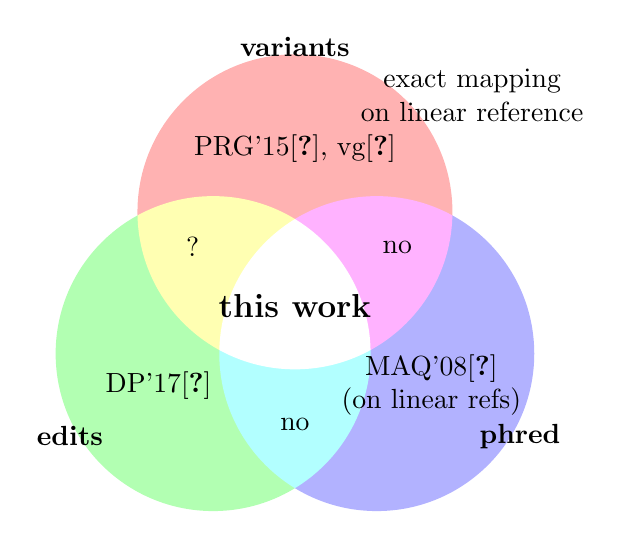
\begin{tikzpicture}
		\begin{scope}[blend group = lighten]
			\fill[red!30!white]   ( 90:1.2) circle (2);
			\fill[green!30!white] (210:1.2) circle (2);
			\fill[blue!30!white]  (330:1.2) circle (2);
		\end{scope}
		
		% labels
		\node at (90:3.3)    {\textbf{variants}};
		\node at (210:3.3)   {\textbf{edits}};
		\node at (330:3.3)   {\textbf{phred}};
		
		% 0 intersect (outside)
		\node [text width=3cm, align=center] at (50:3.5)    {exact mapping \\ on linear reference};
		
		% 1 intersect
		\node at (90:2)      {PRG'15\cite{dilthey2015improved}, vg\cite{VGtool}};
		\node at (210:2)     {DP'17\cite{rautiainen2017aligning}};
		\node [text width=3cm, align=center] at (330:2)     {MAQ'08\cite{maq2008mapping} \\ (on linear refs)};
		
		% 2 intersect
		\node at (150:1.5)   {?};   % between variants and edits
		\node at (270:1.5)   {no};  % between edits and phred
		\node at (30:1.5)    {no};  % between variants and phred
		
		% 3 intersect	
		\node [font=\large] {\textbf{this work}};
	\end{tikzpicture}
	\caption{Comparison of existing mapping approaches based on supported sources of uncertainty: different weighting of reference variants, edit distance minimization to reference, and query phred values} \label{fig:VennComparison}
\end{figure}

\fxwarning{Add columns to the comparison table: complexity, short/long read, single/pair-end, dataset, multiple reads (\eg extend from seed-and-extend, MSA)}
\fxwarning{Add rows to the comparison table: check with https://genome.cshlp.org/content/27/5/665.full.pdf\cite{paten2017genome}}
\begin{table*}
	\centering
	\begin{tabular}{lccccccccc}
		\toprule
		\bf{tool}  & \specialcell{\bf{reference}\\ \bf{graph}}  & \bf{variants}  & \bf{edits}  & \bf{phred}  & \specialcell{\bf{quality}\\ \bf{score}}  & \bf{probabilistic}  & \specialcell{\bf{no}\\ \bf{adhoc}}  & \bf{efficiency}  & \bf{evals} \\
		% tool+citation									& graph			& vars	& edits	& phred	&qual.score & prob	& not adhoc	& fast	& evals
		\midrule                                                                                                                    
		Smith-Waterman'81 \cite{smith1981comparison}	& linear		& \n	& \y	& \n	& \n	& \n			& \y	& \y	& ?		\\
		MAQ'08 \cite{maq2008mapping}					& linear		& \n	& (\n)	& \y	& \y	& \y (approx.)	& \y	& \y	& ?		\\
		Bowtie2'12 \cite{langmead2012fast}				& linear		& \n	& \y	& \n	& ?		& \n (ED)		& ?		& \y	& ?		\\ %SOAP'08, BWA'09, TopHat2'13
		Na'09 \cite{na2009alignment}					& linear		& \n	& \y	& \y	& ?		& \y ?			& ?		& ?		& exact alignment when changed DP scores	\\
		LAST'10 \cite{frith2010incorporating}			& linear		& \n	& \n	& \y	& \y	& \y ? 			& \n	& ?		& synth (subst+phred), real (on close specie)		\\
		BWA-MEM											& linear		& \n	& \n	& \n	& ?		& \n (MEM)		& ?		& ?		& ?		\\
%	GenomeMapper'09 \cite{schneeberger2009simultaneous} & ?				& ?		& ?		& ?		& ?		& \n (exact)	& ?		& ?		& ?		\\
		\midrule
		ERG'12 \cite{vijaya2012new}						& linear+variants?& ?	& ?		& ?		& ?		& ?				& ?		& ?		& RNA	\\
		BlastGraph'12 \cite{holley2012blastgraph}		& \y?			& \y	& (\y)	& \n	& \n    & \n			& \n	& \n	& \n	\\
		BWBBLE'13 \cite{huang2013short}					& many linear?	& \y	& ?		& ?		& ?		& ?				& ?		& ?		& ?		\\
		MuGI'14	\cite{danek2014indexes}					& many linear	& \y	& ?		& ?		& ?		& ?				& ?		& ?		& ?		\\
		\bf{GCSA'14} \cite{siren2014indexing}			& DAG*			& \y	& (\y) $\leq$ 3 & \n & \n & \n			& \y	& (\y) when ED is small	& mapping and variation on HG		\\
		HISAT2'15 \cite{kim2015hisat,siren2014indexing,langmead2012fast}
														& DAG*?			& \y	& ?		& \n	& ?		& ?				& ?		& \y	& \n?		\\
		PRG'15 \cite{dilthey2015improved}				& DAG			& \y	& (\n)	& \n	& \n	& ?				& \n	& \n	& only MHC genotypes	\\
		\bf{deBGA'16} \cite{liu2016debga}				& de Bruijn Graph& \y	& \n	& \n	& ?		& \n			& ?		& \y	& sim and real on HG		\\
		\bf{BGREAT'16} \cite{limasset2016read}			& DAG			& \y	& subst	& \n	& \n	& \n			& \n	& \y	& too simple \\
		Gramtools'16 \cite{maciuca2016natural}			& DAG			& \y	& \n	& \n	& \n	& \n			& \n	& \y	& \n	\\
		\bf{partis'16} \cite{ralph2016consistency}		& linear HMMs	& \y	& subst	& \n	& \n	& \y			& (\y)	& \n	& VDJ annotation	\\
		DP'17 \cite{rautiainen2017aligning}	(no tool)	& \y			& \y	& \y	& \n	& \n	& \n (ED)		& \y	& \n	& \n	\\
		Graphtyper'17 \cite{eggertsson2017graphtyper}	& DAG			& \y	& 1subst& \n	& \n 	& max.match		& ?		& \y	& only genotypes	\\
		VG'17 \cite{VGtool,paten2017genome,garrison2018variation}	& \y & \y	& \n	& \n	& ?	 	& \n (MEM)		& ?		& \y	& HG?	\\
		%FORGe'18 \cite{pritt2018forge}(preprint)		& DAG?			& \y	& ?		& ?		& ?		& ?				& ?		& ?		& ?		\\
		\bf{IGoR'18} \cite{marcou2018high}				& ?				& \y	& subst	& \n	& ?		& \n (ED)		& ?		& ?		& VDJ		\\
		\bf{BrownieAligner'18} \cite{Heydari2018}		& \y			& \y	& \y	& \n	& ?		& ?				& ?		& ?		& 		\\
		\bf{\tool}										& \y			& \y	& \y	& \y	& \y 	& \y			& \y 	& Dijkstra ($L N$ nodes, $L M$ edges)	& VDJ		\\
		\bottomrule
	\end{tabular}
	\caption{Comparison of existing mapping approaches (separate aligning steps not included).
		Edits are insertions, deletions and substitutions.
		MAQ accounts for edits after mapping.
		PRG accounts for edits after mapping and linearization.
		Only evaluated features are included. The DAG* can be extended to general graph.
	}
	\label{table:comparison}
\end{table*}

Multiple Genome Index(MuGI'14)

The Na'09 paper\cite{na2009alignment} aligns a read to another read.
They modify the edit penalties based on quality scores.
The evals are just counting how often the standard DP finds exactly the same alignment as the modified DP with the quality scores finds.

LAST'10\cite{frith2010incorporating} aligns a read to a genome allowing only for mismatches because of sequencing or wrong mapping.
The evals include both synthetic and real data.
In the simulated tests, they sample 36bp fragments with different levels of random substitutions (modeling the biological variation) and add noise from real phred values.
The real setting is xeno-mapping of reads from one specie to the genome of another closely related:
	firstly different sets of edit penalties are estimated, then three experiments are conducted: accounting for phreds, phreds+edits, phreds+edits+gaps.

The BlastGraph'12\cite{holley2012blastgraph} tool maps using seed hashing and aligns to the left and right of the seeds using DP minimizing edit distance.
It is evaluated on DBGs built using a 10K, 100K and 100K reads out of approx. 4M Illumina single-end 36nb reads (sra:DRR000096).
The edits compensate for technical noise but not for biological noise. The eval does not include bio variability.

Generalized compressed suffix array'14 (GCSA) is a BWT extention to graphs.
In order to support edits, full set of possible edits should be generated in the index.
It is built from a reference genome + known variation or by a multiple sequence alignment.
Indexes supporting ED of $\leq$ 0, 1, 2 and 3 are compared to RLCSA (Find and Locate) and BWBBLE (Find) on HG.
Evaluated on the Variation dataset'13\cite{}.
They find out that with increasing the allowed ED, mapping on the graph stops finding more or more unique mappings than on the linear reference (allowing for the same ED).

PRG'15\cite{dilthey2015improved} constructs a graph with edge probabilities by chopping reads to kmers. Then the whole reads are mapped to the graph and the two most probable haplotypes. This means that the reads are not mapped to an independent reference genome.

Gramtools'16\cite{maciuca2016natural} uses BWT to represent variations of the reference. Evaluated for speed not accuracy.

deBGA'16 \cite{liu2016debga} indexes a DBG and introduces a graph-based seed-and-extension algorithm.
``Generally, seed-and-extend aligners consist of two steps:
(i) seeding: the inference of putative read positions (PRPs) from the matches (hits) of tokens (seeds) between the read and reference genome;
and (ii) extension: alignment of the read to the region surrounding each PRP to determine the most likely read position(s)''
``One of the major bottlenecks faced by this approach is how to handle repetitive genomic regions, even in the context of a single genome,
for example, over 50\% of the human genome comprised repeats''
The evals measure the sensitivity and accuracy for read alignment against a single genome using simulated and real pair-end reads.
Compared to Bowtie2, BWA, BWA-MEM, STAR, SeqAlto and GEM.

ERG'16 \cite{vijaya2012new}.

BGREAT'16\cite{limasset2016read} maps single-end reads on DBGs using an exhaustive solution and a greedy speedup.
Evals consist of comparing mapping percentable on contigs vs the graph, calculating percentage of reads that map on branching paths.
The accuracy evals are only with sythetic reads with sequencing errors from HG being mapped on the same HB DBG.
Could compare only to BlastGraph but it was too unstable.
We subsume this method as the DBG can be converted to \tool.

Partis'16\cite{ralph2016consistency} precomputes the structure of a set of separate linear HMM for each VDJ recombination.
Then, based on the set of input sequences (\eg reads) it estimates allele usage probs, transition probs and emission probs and annotates each sequence by VDJ alleles.
Given a VDJ distribution and priors on gap size, naive sequences are simulated after which they are mutated (similar to BCR) into a set of sequences of a clonal family (using TreeSim).
Partis does inference by finding a path in the HMM that has maximum probability to generate a single or multiple sequences (multi-HMM).
The V, D and J allele correctness is compared to IMGT, IgBLAST, iHMMunealign and ighutil. Uses SW alignment.

Graphtyper'17\cite{eggertsson2017graphtyper} creates a DAG out of a reference and a set of variants.
Mapping is by hashing kmers (seed-and-extend) which are extracted from a read with 1bp overlap, then extending the seeds of overlapping kmers on the reference, then BFS through the graph structure of overlapping kmers (without any mistakes for now), then extracting kmers with 1 mistake from a read (and its reverse complement) that overlaps by 1bp. Evaluated are only genotype calls but not the alignments.

FORGe'18\cite{pritt2018forge} studies the drawbacks and trade-offs between accuracy and overhead when adding more reference genomes to the graph.
They suggest a method for scoring variants based on the effect on accuracy and the computational overhead and deciding which to add to the graph.
Compared to HISAT2, ERG,

IGoR'18\cite{marcou2018high} has 3 regimes: SW alignment, infer a model and evaluating sequence statistics. Compares to Partis and MiXCR using their own simulated data (instead of reusing). It does SW alignment.

BrownieAligner'18\cite{Heydari2018} works on de Bruijn graphs.
Claims alignment optimality but depends on initial heuristic seeding.
A Markov Model is built by aligning the reads on the graph, and then used for heuristically pruning the spurious paths. It captures more long-distance relationships than $k$.
Seems to use a cutoff of 2 indels for a banded DP.
Its scores (+1,-1,-3) are not general and what is most important, the matching score should be >0 (as commented in the code).
No phreds support. No probabilistic interpretation.
In the implementation, they perform DFS with a stack instead of priority queue (as shown in the paper).
They evaluate on simulated and on real reads from one genome: reads are simulated using ART tool\cite{huang2011art}, and the real reads true locations are assumed to be the ones found by bwa (no variant data).
B\&B speeds-up DFS between 1.1 times and 4-5 times.

In\cite{garrison2018variation} VG is evaluated by mapping simulated reads from a 150bp pair-end reads

As visualized on figure \ref{fig:VennComparison}, existing approaches regard some of the mentioned uncertainty sources but do not unify them in order to extract full advantage of the available data.

\section{Problem Statement} \label{sec:problem-statement}

\tool phrases alignment as a probabilistic inference task that we introduce and motivate in this section. The inference task is based on a generative model that specifies how reads are generated. A mathematically precise formulation of this generative model ensures that \tool solves the correct alignment task.

\para{Notation}
\cref{tab:notation} provides a summary of notation used in this work.
The first two parts of \cref{tab:notation} provide a quick reference for the notation introduced in this section.
For now, we only note that we distinguish sets of instances (\eg $\genomes$), random variables inducing a distribution over these sets (\eg $G$), and instances of random variables (\eg $g$).

The last part of \cref{tab:notation} summarizes notation we use without further comments.
The only non-standard notation is $\genome\llbracket i \rrbracket$ (and $\genome\llbracket i \shortcolon j \rrbracket$), which we use to indicates the positions at which a given read could align.
Formally, we can interpret $\genome\llbracket i \rrbracket$ as the tuple $(\genome,i)$.

% We use standard, but explicit notation to indicate the probability of events. For example, to indicate the probability of alignment $a$, conditioned on observing the read $s$, we write

% Here, the subscripts $A,S^\gread$ explicitly indicate that the probability is over the joint distribution of $A$ and $S^\gread$.
% We note that this notation allows $A$ and $S^\gread$ to be correlated.

% The symbol $\graph$ stands for graph representing a random variable over genome segments. 

\begin{table}
	\centering
	\small
	\begin{tabular}{ c c c c }
		& Set & Random Variable & Instance \\
		Genome & $\genomes$, $\genomes^\gcore$, $\genomes^\gmut$ & $\genomeRV$, $\genomeRV^\gcore$, $\genomeRV^\gmut$ & $\genome$, $\genome^\gcore$, $\genome^\gmut$ \\
		Alignment & $\alignments$ & $\alignmentRV$ & $\alignment$, $\alignment^\star$ \\
		Genome Segment & $\segments$, $\segments^\gread$ & $\segmentRV$, $\segmentRV^\gread$ & $\segment$, $\segment^\gread$ \\
		Start of segment & $\{0,\dots,\abs{\genome}-1 \}$ & $\startInGenomeRV$, $\startInGenomeRV^\gmut$ & $\startInGenome$, $\startInGenome^\gmut$
	\end{tabular} \\
	%\fullline \\
	\begin{tabular}{ l c }
		\\[-1em] \hline \\[-1em]
		% Meaning of superscript & Usages \\
		Superscript indicating core genome & $^\gcore$ \\ % , as in $\genomes^\gcore$, $\genomeRV^\gcore$, $\genome^\gcore$
		Superscript indicating mutated genome & $^\gmut$ \\ % , as in $\genomes^\gmut$, $\genomeRV^\gmut$, $\genome^\gmut$ / $\startInGenomeRV^\gmut$, $\startInGenome^\gmut$
		Superscript indicating read of genome segments & $^\gread$ \\ % , as in $\segments^\gread$, $\segmentRV^\gread$, $\segment^\gread$
		\\[-1em] \hline \\[-1em]
		Letter at \nth{i} position of genome $\genome$ ($0$-based indexing) & $\genome[i]$ \\
		Position $i$ in genome $\genome$ & $\genome \llbracket i \rrbracket$ \\
		Letters/Positions $i$ (inclusive) to $j$ (exclusive) of genome $\genome$ & $\genome[i \shortcolon j]$, $\genome \llbracket i \shortcolon j \rrbracket$ \\
		Length of genome or segment & $\abs{\genome}$, $\abs{\segment}$ \\
		Set of paths of length $L$ in graph $\graph$ & $\paths{L}{\graph}$
	\end{tabular}
	\caption{Summary of notation.}
	\label{tab:notation}
\end{table}

\para{Inspiration: Complete Genomes Model}
Our generative model is inspired by a model of biological reality, depicted in the first column of \cref{fig:models}.

It starts from a random variable $\genomeRV$ over the set $\genomes = \{\genome_i\}_{i \in \mathcal{I}}$ of haploid genomes occurring in the population under consideration.
The genomes in $\genomes$ exhibit both small-scale and large-scale variations appearing in the population.
Small-scale variations include de-novo mutations and other rare mutations, while large-scale variations capture common mutations in the population that typically span multiple base pairs.
The distribution of the random variable $\genomeRV$ captures the probability of each genome $\genome$.
We note that this distribution is typically not uniform, as some variations are more common than others.
As a consequence, ignoring the distribution of $\genomeRV$ (as done, \eg by the Smith-Waterman algorithm) will necessarily lead to loss of information.

The model first samples a genome $\genome$ from $\genomeRV$.
Then, it sequences $\genome$, resulting in a read $\segment^\gread$ of a predetermined length $L$.
Sequencing consists of (i)~randomly chopping the genome into smaller segments, (ii)~discarding segments shorter than $L$ and selecting one remaining segment $\segment$ of length at least $L$ to read, and (iii) reading the first $L$ letters in $\segment$, resulting in $\segment^\gread$.
In general, $\segment \neq \segment^\gread$ even if the length of $\segment$ is $L$, as reading is noisy and may introduce \emph{read errors}.

We assume the model does not only report the read $\segment^\gread$, but also the probability of reading each letter correctly.
Typically, this probability is represented as a phred quality score \cite{ewing_base-calling_1998}:
$$Q_i := -10 \cdot \log_{10}\Pr{\text{error reading \nth{i} letter}},$$
However, we work with phred probabilities instead, denoted by
$$
\pphred{i} := \Pr{\text{correctly reading \nth{i} letter}}.
$$


\subsection{Our Model: Core Genomes Model} \label{sec:generative-model}
%In this section, we describe the generative model underlying our inference task.
Instantiating the Complete Genomes Model in practice is impossible; we typically cannot even enumerate all genomes in $\genomes$.
Instead, we introduce the Core Genomes Model, which starts from a random variable $\genomeRV^\gcore$ over a set $\genomes^\gcore$ of \emph{core genomes}.
In contrast to $\genomes$, the core genomes in $\genomes^\gcore$ only capture the large-scale variations appearing in the population.

\para{Mutations}
Our model introduces small-scale variations by first sampling a core genome $\genome^\gcore$ from $\genomeRV^\gcore$ and then mutating it.
To mutate $\genome^\gcore$, our model copies it letter by letter, generating a mutated genome $\genome^\gmut$.
When the model is about to copy the \nth{i} letter of $\genome^\gcore$, it probabilistically decides to (i)~insert a new letter (insertion), (ii)~skip this letter (deletion), (iii)~copy the letter incorrectly (edit), or (iv)~copy the letter correctly (copy).

\begin{figure}
	\lstinputlisting[language=MyPython,caption={Code for mutating a core genome.},label={lst:mutate-minified}]{code/mutate_minified.py}
\end{figure}

\cref{lst:mutate-minified} shows an algorithmic description of this mutation process.
It iterates over the positions \texttt{i} in $\genomes^\gcore$ and and in every step determines all possible actions (\crefrange{line:mutate-actions-def}{line:mutate-actions-select}).
Each action consists of a probability for that action, an action type (insertion, deletion, edit, copy), and the letter produced by this action ($\epsilon$ indicates no letter, for deletions).
Unless the action is a deletion, \cref{lst:mutate-minified} appends the new letter to the mutated genome (\crefrange{line:mutate-del-check}{line:mutate-no-del}).
Then, unless the action is an insertion, \cref{lst:mutate-minified} advances the read pointer (\crefrange{line:mutate-ins-check}{line:mutate-no-ins}).

For simplicity of presentation, \cref{lst:mutate-minified} assumes that each action type occurs with a constant probability at every position. 
In addition, it assumes that the new letter for insertions and edits is selected uniformly at random from all letters, \ie each letter has a probability of $\pins/4$ to be inserted.
Likewise, the process selects the new letter for edits uniformly at random from all letters different from the current one, \eg copying letter $A$ yields (edited) letter $C$, $G$, or $T$ with a probability of $\ped/3$, respectively.
It is straightforward to extend \cref{lst:mutate-minified} to allow for position-dependent action probabilities, and for a selection of new letters according to a different distribution.

In \cref{line:mutate-return}, \cref{lst:mutate-minified} does not only return the mutated genome $\genome^\gmut$, but also its mutation history \texttt{mutations}, constructed in \cref{line:mutate-history}.
For every step in the mutation process, the history records (i)~the current position of the read pointer consisting of $\genome^\gcore$ and \texttt{i}, (ii) the action type (\texttt{action}), and (iii)~the generated letter (\texttt{letter}).

\para{Sequencing}
After determining $\genome^\gmut$, our model sequences it according to the following steps (these steps formalize the sequencing process described in the Complete Genomes Model).

First, it selects a starting point $\startInGenome$ in $\genome^\gmut$ by sampling from a random variable $\startInGenomeRV$ describing the distribution over all possible starting points.
To avoid reads of length less than $L$, $\startInGenomeRV$ must never select one of the last $L-1$ positions of $\genome$.

Second, our model determines the segment $\segment := \genome[\startInGenome \shortcolon \startInGenome+L]$.
We note that unlike the Complete Genomes Model, our model does not produce longer segments than $L$ at this stage.
Since the read only depends on the first $L$ letters of $\segment$, this simplification does not affect the behavior of our model.

\begin{figure}
	\lstinputlisting[language=MyPython,caption={Code for reading a sequence.},label={lst:read-minified}]{code/read_minified.py}
\end{figure}

Finally, our model reads $\segment$ letter by letter in order to produce $\segment^\gread$.
We provide an algorithmic description of the read process in \cref{lst:read-minified}.
For every letter, the model may (i)~read it correctly with probability \texttt{1-p\_error}, or (ii)~read it incorrectly with probability \texttt{p\_error}.
Analogously to the mutation process, for simplicity of presentation, \cref{lst:read-minified} assumes constant error probabilities and a selects erroneous letters uniformly at random.
Likewise, \cref{line:read-return} does not only return the sequenced read $\segment^\gread$, but also its read error history \texttt{errors}, constructed in \cref{line:read-history}.
For every read letter, the history records (i)~the current position of the read pointer, (ii)~the action type, and (iii)~the generated letter.

% We assume that if $\genomes^\gcore$ and the mutation process are selected appropriately, capturing large-scale and small-scale variations respectively, then $\genome^\gmut$ follows the same distribution as $\genome$ sampled from $\genomes$.
% Under this assumption, the Core Genomes Model is equivalent to the Complete Genomes Model.

\begin{figure}
	\centering
	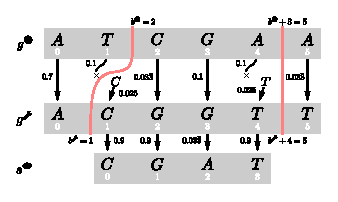
\includegraphics[width=0.99\linewidth]{figures/edit-example}
	\caption{Generation of a read $\segment^\gread=CGAT$ from core genome $\genome^\gcore=ATCGAA$ by editing and sequencing. Arrows indicate copied letters ($\pcopy=0.7$) or edited (dashed arrow; $\ped=0.1$), inserted (arrow starting from a new letter; $\pins=0.1$), or deleted (arrow to x; $\pdel=0.1$). During sequencing, we assume a phred probability of $\pphred{i} = 0.9$ at every position $i$.}
	\label{fig:alignment-full}
\end{figure}

\para{Example}
\cref{fig:alignment-full} shows the full process of generating $\segment^\gread$ on a concrete example.
The model first selects a core genome $\genome^\gcore=ATCGAA$.
Then, it copies $\genome^\gcore$ letter by letter, generating the mutated genome $\genome^\gmut=ACGGTT$.
The numbers in \cref{fig:alignment-full} indicate the probabilities of each action.
Overall, the probability of generating $\genome^\gmut$ from $\genome^\gcore$, according to the depicted actions, is $0.7 \cdot 0.1 \cdot 0.025 \cdot 0.03\bar{3} \cdot 0.1 \cdot 0.1 \cdot 0.025 \cdot 0.03\bar{3} \approx 5 \cdot 10^{-10}$.
We note there are other actions that can also generate $\genome^\gmut$ from $\genome^\gcore$, \eg instead of editing $C$ to $G$, the model could delete $C$ and insert $G$.

After generating $\genome^\gmut$, the model selects a starting position $\startInGenome^\gmut=1$ and copies the $L=4$ letters $\genome^\gmut[1 \shortcolon 5]$ to generate $\segment^\gread$.
The probability of generating $\segment^\gread$ from $\genome^\gmut$ is $0.9 \cdot 0.9 \cdot 0.03\bar{3} \cdot 0.9 \approx 2.4 \cdot 10^{-2}$.

\subsection{Alignment as an Inference Task} \label{sec:alignment}
In this section, we define the alignment task as an inference task in the generative model introduced in \cref{sec:generative-model}.
Our generative model induces a genome alignment task: Given a read $\segment^\gread$, determine its generation history consisting of the mutation history and the read error history leading to $\segment^\gread$.

Generally, given the mutation history and the read $\segment^\gread$, the read error history can be reconstructed.
In addition, the mutation history describes the generation of the full $\genome^\gmut$, even though $\segment^\gread$ may only provide information about the generation of $\genome^\gmut[\startInGenome \shortcolon \startInGenome + L]$. 
Therefore, we define the alignment $\alignment$ of $\segment^\gread$ to be its mutation history, restricted to positions $\startInGenome^\gmut$ to $\startInGenome^\gmut + L$.
%In terms of the algorithmic description in \cref{lst:mutate-full}, $\alignment = \texttt{history}[\startInGenome^\gmut:\startInGenome^\gmut+L]$.

\para{Example}
In \cref{fig:alignment-full}, alignment only considers the mutations occurring
between the red lines. Concretely, \cref{fig:alignment-full} induces alignment
$\alignment$, given by 
\begin{align*}
&(\genome^\gcore\llbracket 2 \rrbracket,\text{ins},C),(\genome^\gcore\llbracket 2 \rrbracket,\text{edit},G), (\genome^\gcore\llbracket 3 \rrbracket,\text{copy},G),\\
&(\genome^\gcore\llbracket 4 \rrbracket,\text{del},\epsilon),(\genome^\gcore\llbracket 5 \rrbracket,\text{ins},T).
\end{align*}

We note that $\alignment$ does not include the deletion of $T$, as it occurred before generating the first letter from $\segment^\gread$.
Likewise, it does not include deletions that occur after generating the last letter from $\segment^\gread$.

\para{\acs{map} Alignment}

Given only $\segment^\gread$ from \cref{fig:alignment-full}, there are more likely alignments than $\alignment$.
For example, instead of deleting $\alignment$ from $\genome^\gcore$ and inserting $T$ into $\genome^\gmut$, editing $A$ to $T$ would be a more likely explanation.
Generally, we can not hope to always identify the true alignment of a read, but we can determine the most likely alignment $\alignment^\star$, given the read $\segment^\gread$. This corresponds to \acf{map} estimation, and can be written as:
\begin{align} \label{eq:MAP-alignment}
	\alignment^\star = \argmax_{\alignment} \Pr{\alignmentRV=\alignment \mid \segmentRV^\gread = \segment^\gread}
\end{align}

In \cref{eq:MAP-alignment}, we are using random variables $\alignmentRV$ and $\segmentRV^\gread$ which are correlated: $\alignmentRV$ is the alignment of $\segmentRV^\gread$.

% \begin{figure}	
% \begin{tikzpicture}
% 	node distance=2.5cm, % Minimum distance between two nodes. Change if necessary.
% 	every state/.style={ % Sets the properties for each state
% 		semithick,
% 		fill=gray!10},
% 	initial text={}, % No label on start arrow
% 	double distance=2pt, % Adjust appearance of accept states
% 	every edge/.style={ % Sets the properties for each transition
% 		draw,
% 		->,>=stealth’, % Makes edges directed with bold arrowheads
% 		auto,
% 	semithick}

% 	\node[state, initial] (q1) {$q_1$};
% 	\node[state, right of=q1] (q2) {$q_2$};
% 	\node[state, right of=q2] (q3) {$q_3$};
% 	\node[state, right of=q3] (q4) {$q_4$};
% 	\node[state, accepting, right of=q4] (qN) {};

% 	\draw (q1) edge[loop above] node {\tt A,C,G,T} (q1);
% 	\draw (q1) edge[] node {\tt G} (q2);
% 	\draw (q1) edge[bend right=60] node {\tt A,C,G,T,$\epsilon$} (q2);

% 	\draw (q2) edge[loop above] node {\tt A,C,G,T} (q2);
% 	\draw (q2) edge[] node {\tt A} (q3);
% 	\draw (q2) edge[bend right=60] node {\tt A,C,G,T,$\epsilon$} (q3);

% 	\draw (q3) edge[loop above] node {\tt A,C,G,T} (q3);
% 	\draw (q3) edge[] node {\tt T} (q4);
% 	\draw (q3) edge[bend right=60] node {\tt A,C,G,T,$\epsilon$} (q4);

% 	\draw (q4) edge[loop above] node {\tt A,C,G,T} (q4);
% 	\draw (q4) edge[] node {\tt $\epsilon$} (qN);
% \end{tikzpicture}
% \end{figure}

% \para{MAP vs MLE} \todo{this paragraph does not fit here. I don't think it is relevant, can probably be deleted}
% In the context of MAP and MLE optimization during inference, the observed data is the query read and the mapping parameter is the resulting alignment.
% In case of a uniform distribution of the genomes in the core model, MAP mapping is equivalent to MLE mapping.
% Not weighting the starting positions in the graph models is indirectly stating some (possibly not uniform) prior distribution on the genomes and their positions.
% In order to translate a known core genomes prior of the genomes to the graph model, the edge weights have to be chosen or learned appropriately.


% \begin{itemize}
% 	\item desirable properties
% 	\item $3$ sources of uncertainty
% \end{itemize}

\section{Graph Model} \label{sec:graph-model}
In this section, we introduce a graph representation of the core genomes that
enables us to efficiently solve the inference problem introduced in \cref{sec:alignment}.
The third column in \cref{fig:models} shows the resulting generative model.

Variation graphs provide a succinct encoding of all possible segments of core genomes.
Conventional variation graphs have shown great promise in capturing large-scale variations that linear references cannot represent \cite{VGtool,paten2017genome,garrison2018variation}.
Here, we generalize these variation graphs to our probabilistic setting.

\begin{figure*}
	\begin{minipage}{0.7\linewidth}
		\begin{tikzpicture}[
		node distance=0.5cm,
		myletter/.style={letter,scale=0.9,text width=2em,inner sep=0pt,align=center},
		myarrow/.style={arrow}
	]
	% vertex positions
	\def \vd {0.8}
	\pgfmathsetmacro{\leftx}{3}
	\pgfmathsetmacro{\middlex}{\leftx+4*\vd}
	\pgfmathsetmacro{\rightx}{\leftx+7*\vd}

	% GENOMES

	\node[] at (0, 0.9) (g1) {$\genome_1^\gcore=$ \textcolor{my-full-blue}{$AAC$} $CCG$ \textcolor{my-full-blue}{$AAC$}};
	\node[] at (0, 0.3) (g2) {$\genome_2^\gcore=$ \textcolor{my-full-blue}{$AAC$} $CCG$ \textcolor{my-full-purple}{$GGT$}};
	\node[] at (0,-0.3) (g3) {$\genome_3^\gcore=$ \textcolor{my-full-purple}{$GGT$} $CCG$ \textcolor{my-full-blue}{$AAC$}};
	\node[] at (0,-0.9) (g4) {$\genome_4^\gcore=$ \textcolor{my-full-purple}{$GGT$} $CCG$ \textcolor{my-full-purple}{$GGT$}};

	% ARROW

	\node[inner sep=0pt,above right,anchor=center] at (2.2,0) {\includegraphics[scale=1]{figures/arrow}};

	% GRAPH-LEFT

	\node[myletter] at (\leftx, 0) (left) {$v_0$};

	\path (left)
		 ++(\vd,0.6) node[myletter,my-full-blue] (left-AAC-1) {$v_1$}
		 ++(\vd,0) node[myletter,my-full-blue] (left-AAC-2) {$v_2$}
		 ++(\vd,0) node[myletter,my-full-blue] (left-AAC-3) {$v_3$};
	
	\path (left)
		 ++(\vd,-0.6) node[myletter,my-full-purple] (left-GGT-1) {$v_4$}
		 ++(\vd,0) node[myletter,my-full-purple] (left-GGT-2) {$v_5$}
		 ++(\vd,0) node[myletter,my-full-purple] (left-GGT-3) {$v_6$};

	% GRAPH-MIDDLE

	\path (\middlex,0) node[myletter] (CCG-1) {$v_7$}
		++(\vd,0) node[myletter] (CCG-2) {$v_8$}
		++(\vd,0) node[myletter] (CCG-3) {$v_9$};
	
	% GRAPH-RIGHT

	\path (\rightx, 0.6) node[myletter,my-full-blue] (right-AAC-1) {$v_{10}$}
		   ++(\vd,0) node[myletter,my-full-blue] (right-AAC-2) {$v_{11}$}
		   ++(\vd,0) node[myletter,my-full-blue] (right-AAC-3) {$v_{12}$};

	\path (\rightx,-0.6) node[myletter,my-full-purple] (right-GGT-1) {$v_{13}$}
		++(\vd,0) node[myletter,my-full-purple] (right-GGT-2) {$v_{14}$}
		++(\vd,0) node[myletter,my-full-purple] (right-GGT-3) {$v_{15}$};
	
	% GRAPH EDGES

	\draw[myarrow,my-full-blue] (left) -- node[above] {$A$} (left-AAC-1);
	\draw[myarrow,my-full-blue] (left-AAC-1) -- node[above] {$A$} (left-AAC-2);
	\draw[myarrow,my-full-blue] (left-AAC-2) -- node[above] {$C$} (left-AAC-3);

	\draw[myarrow,my-full-purple] (left) -- node[above] {$G$} (left-GGT-1);
	\draw[myarrow,my-full-purple] (left-GGT-1) -- node[above] {$G$} (left-GGT-2);
	\draw[myarrow,my-full-purple] (left-GGT-2) -- node[above] {$T$} (left-GGT-3);

	\draw[myarrow] (left-AAC-3) -- node[right,pos=0.3] {$C$} (CCG-1);
	\draw[myarrow] (left-GGT-3) -- node[right,pos=0.3] {$C$} (CCG-1);
	\draw[myarrow] (CCG-1) -- node[above] {$C$} (CCG-2);
	\draw[myarrow] (CCG-2) -- node[above] {$G$} (CCG-3);

	\draw[myarrow,my-full-blue] (CCG-3) -- node[left,pos=0.7] {$A$} (right-AAC-1);
	\draw[myarrow,my-full-blue] (right-AAC-1) -- node[above] {$A$} (right-AAC-2);
	\draw[myarrow,my-full-blue] (right-AAC-2) -- node[above] {$C$} (right-AAC-3);

	\draw[myarrow,my-full-purple] (CCG-3) -- node[left,pos=0.7] {$G$} (right-GGT-1);
	\draw[myarrow,my-full-purple] (right-GGT-1) -- node[above] {$G$} (right-GGT-2);
	\draw[myarrow,my-full-purple] (right-GGT-2) -- node[above] {$T$} (right-GGT-3);
\end{tikzpicture}
		\caption{Variation graph capturing genomes $\{\genome_1, \genome_2, \genome_3, \genome_4\}$.}
		\label{fig:deterministic-variation-graph}
	\end{minipage}\hspace{0.04\linewidth}
	\begin{minipage}{0.25\linewidth}
		\centering
		
\includegraphics[width=0.8\linewidth]{figures/partition}
		\caption{Concretization of paths of length $L$.}
		\label{fig:partition}
	\end{minipage}
\end{figure*}

\para{Variation Graphs}
\cref{fig:deterministic-variation-graph} shows a set of genomes $\genomes$ (left) encoded by a conventional variation graph $\graph$ (right).
The graph $\graph=(V,E)$ consists of vertices $V$ and edges $E$ and is equipped with edge labels $\labels \colon E \to \{A,C,G,T\}$.
Thus, each path $\graphpath=e_1,\dots, e_n$ in $\graph$ spells a genome segment by $\labels(\graphpath)=\labels(e_1) \cdots \labels(e_n)$, where $\cdot$ denotes string concatenation.

In addition, $\graph$ is equipped with a position map $\position \colon E \to \mathcal{P}(\genomes \times \mathbb{N})$ which annotates each edge with a set of positions in the genomes.
For example, $\position((v_0,v_1))=\{\genome_1\llbracket 0 \rrbracket,\genome_2\llbracket 0 \rrbracket\}$, as the edge between $v_0$ and $v_1$ represents the first letter of the first two genomes.
In practice, we may not know the positions referred to by each vertex $v$.
In this case, we simply annotate $v$ with basic information about its position,
such as its approximate location in a reference genome.

When given a read $\segment^\gread$, existing graph alignment tools aim to find a path $\graphpath$ in $\graph$ that spells $\segment^\gread$, or a slightly edited version of it.
The annotations on the graph's vertices then allow us to identify the (set of) positions $\segment^\gread$ most likely originates from.

\para{Concrezitation of Paths}
Every path $\graphpath$ in $\graph$ represents one or multiple segments of genomes.
We capture these segments by a concretization function $\gamma$ taking as argument a path $\graphpath$ consisting of edges $e_i$.
Given $\graphpath$, $\gamma$ returns the set of all possible segments $\graphpath$ may represent, where each segment is encoded as a sequence of positions, determined by the position map $m$:
\begin{align*}
	\gamma(e_1, \dots, e_L) = \{p_1, \dots, p_L \mid p_i \in \position(e_i)\}
\end{align*}

\para{Compression by Variantion Graphs}
\cref{fig:partition} visualizes the concretization of paths of length $L$.
Green circles (\coloredcircle{my-full-green}) represent segments present in $\genomes$, while orange circles (\coloredcircle{my-full-orange}) represent spurious segments.
\cref{fig:partition} shows that the concretization of every path of length $L$ contains at least one segment from $\genomes$.
This is necessary when aligning reads of length $L$ since otherwise, alignment on $\graph$ may select a spurious path that does not reflect an existing genome segment.
Likewise, \cref{fig:partition} does not show any genome segment of length $L$ that is not captured by concretizing some path.
Otherwise, some reads of length $L$ could never be aligned correctly in $\graph$.

When $\graph$ captures these two properties for every length $L'<L$, we say $\graph$ \emph{non-deterministically $L$-compresses} the set of genomes $\genomes$.
This ensures that (i)~any path selected by alignment can be interpreted in the genomes and (ii)~any read can be aligned on $\graph$.
The formal definition is that for all lengths $L' \leq L$:
\begin{align}
	\forall \graphpath \in \paths{L'}{\graph}. \exists \genome \in \genomes, \startInGenome < \abs{\genome}-L'. \genome \llbracket \startInGenome \shortcolon \startInGenome + L' \rrbracket \in \gamma(\graphpath) \label{eq:compress-non-deterministic-precise} \\
	\forall \genome \in \genomes, \startInGenome < \abs{\genome}-L'. \exists \graphpath \in \paths{L'}{\graph}. \genome \llbracket \startInGenome \shortcolon \startInGenome + L' \rrbracket \in \gamma(\graphpath) \label{eq:compress-non-deterministic-complete}
\end{align}
% \begin{align} \label{eq:compress-non-deterministic}
% \bigcup_{\pi \in \graph} \gamma(\pi) = \left\{ \genome^\gcore\llbracket i \shortcolon i+L' \rrbracket \,\middle|\,
% \genome^\gcore \in \genomes^\gcore,
% 0 \leq i < |\genome^\gcore|-L'
% \right\}.
% \end{align}

% Generally, when aligning reads of length $L$ to a graph $\graph$, we need $\graph$ to $L$-compress the underlying set of core genomes.
% If \cref{eq:compress-non-deterministic-complete} does not hold, \ie $\graph$ does not represent some core genome segments, then some reads cannot be correctly aligned.
% If \cref{eq:compress-non-deterministic-precise} does not hold, \ie $\graph$ contains genome segments that do not occur in the core genomes, alignment on $\graph$ may select a spurious path that was only introduced in the graph model and does not reflect an existing core genome.

\para{Probabilistic Variation Graphs}
In order to account for our generative model, we generalize variation graphs to a probabilistic setting.
To this end, we extend $\graph$ by transition probabilities $\trans \colon E \to [0,1]$ which must induce a probability distribution over all outgoing edges, \ie for all $v \in V$, $\sum_{(v,v') \in E} \trans(v,v')=1$.
Then, the probability of selecting $\graphpath$ is given by $\trans(\graphpath)=\prod_{i=1}^{n} \trans(e_i)$.

In addition, we mark a node $\startNode \in V$ as a distinguished starting node.
Then, all paths $\graphpath=e_1,\dots,e_n$ in $\graph$ must start from $\startNode$, \ie $e_1=(\startNode,v)$ for some $v$.

\para{Compression by Probabilistic Variation Graphs}
To enable alignment on probabilistic variation graphs, it does not suffice if $\graph$ non-deterministically $L$ compresses $\genomes$.
Instead, we must additionally ensure that $\graph$ correctly captures the distribution of $\genomeRV$.
For example, in \cref{fig:partition}, we require that
$$\trans(\pi_3) = \Pr{\genomeRV \llbracket \startInGenomeRV \shortcolon \startInGenomeRV+L' \rrbracket \in \{\coloredcircle[1]{my-full-green},\coloredcircle[2]{my-full-green},\coloredcircle[3]{my-full-orange}\}}.$$

Formally, a probabilistic variation graph $\graph$ \emph{(probabilistically) $L$-compresses} a distribution over genomes $\genomeRV$ if the probability of every path $\graphpath$ of length $L' \leq L$ in $\graph$ matches the probability of the concretization of this path:
\begin{align} \label{eq:compress-probabilistic}
	\trans(\graphpath) = \Pr{\genomeRV\llbracket \startInGenomeRV \shortcolon \startInGenomeRV+L' \rrbracket \in \gamma(\graphpath)} && \forall \graphpath \in \paths{L'}{\graph}
\end{align}

\cref{lem:l-compress-generalize} states that probabilistic L-compression indeed
generalizes deterministic L-compression to the probabilistic setting.

\begin{lemma} \label{lem:l-compress-generalize}
	Assume $\graph$ does not contain edges that may never be used, \ie assume $\forall e \in E. \trans(e)>0$. If $\graph$ probabilistically $L$-compresses a distribution over genomes $\genomeRV$, then $\graph$ non-deterministically $L$-compresses the underlying set of genomes $\genomes$.
\end{lemma}
\begin{proof}
	Let $L' < L$.

	Showing \cref{eq:compress-non-deterministic-precise}: Let $\graphpath = e_1,\dots,e_n \in \paths{L'}{\graph}$. Because $\trans(\graphpath) > 0$ (otherwise there would be an edge that may never be used), and due to \cref{eq:compress-probabilistic}, $\Pr{\genomeRV \llbracket \startInGenomeRV \shortcolon \startInGenomeRV+L' \rrbracket \in \gamma(\graphpath)}>0$. Therefore, there must be at least one $\genome$, $\startInGenome$ with $\genomeRV\llbracket \startInGenomeRV \shortcolon \startInGenomeRV+L' \rrbracket \in \gamma(\graphpath)$.

	Showing \cref{eq:compress-non-deterministic-complete}: Due to \cref{eq:compress-probabilistic}, and because the transition probabilities $\trans$ induce a probability distribution, we have
	\begin{align*}
		\sum_{\pi \in \paths{L'}{\graph}} \Pr{\genomeRV\llbracket \startInGenomeRV \shortcolon \startInGenomeRV+L' \rrbracket \in \gamma(\graphpath)} = \sum_{\pi \in \paths{L'}{\graph}} \trans(\pi) = 1.
	\end{align*}
	Therefore, we know that all genome sequences must be covered by paths in $\graph$.
\end{proof}

\para{Approximate Compression}
In practice, we can only approximately satisfy \cref{eq:compress-probabilistic}.
\todo{Extend probabilistic L-compression to its approximate version}

% We measure the error according to KL divergence. 
% Concretely, we say that $\graph$ \emph{$(L,\epsilon)$-compresses} a distribution over genomes $\genomeRV$ if for all $L' \leq L$: \todo{explain more, if we are to stick with KL divergence}
% \begin{align*}
% 	\E[\Pi \sim \paths{L'}{\graph}]{
% 		\frac{
% 			\trans(\Pi)
% 		}{
% 			\Pr{\genomeRV\llbracket \startInGenomeRV \shortcolon \startInGenomeRV+L'\rrbracket \in \gamma(\Pi)}
% 		}
% 	} \leq \epsilon
% \end{align*}
% This essentially limits KL divergence: $\kld{\graph}{\genomeRV}\leq \epsilon$ (modulo $L$).

\subsection{Generative Graph Model}
\begin{figure}
	\lstinputlisting[language=MyPython,caption={Code for generating a read using the graph model.},label={lst:graph-minified}]{code/graph_minified.py}
\end{figure}

In \cref{lst:graph-minified}, we show an algorithmic description of our
generative model. It starts from an empty read (\cref{line:empty}) and extends
it until it reaches $L$ letters (\cref{line:empty}). In each iteration, it
samples a new edge in the graph (\cref{line:edge}), possibly mutates the letter
associated with this edge (\cref{line:mutate}) and records the resulting action
(\cref{line:record}). Unless the mutation (\cref{line:mutate}) results in a
deletion, the model reads the resulting letter (\cref{line:read}) possibly
resulting in a read error, and appends the resulting letter to the read. In
addition, unless the mutation (\cref{line:mutate}) results in an insertion (in
which case the next letter to be read remains the same), \cref{line:new-state}
updates the current position in the graph.

\subsection{Equivalence of Graph Model and Core Genomes Model}
\todo{Discuss and prove}


\section{Old Graph Model}

Instead of selecting an entire core genome $\genome^\gcore$, we generate a core segment $\segment^\gcore$ of $L$ letters that follows the same distribution as (i)~sampling a core genome $\genome^\gcore$ and (ii)~emitting $L$ letters from a random starting point in $\genome^\gcore$.

To select the core sequence $\seq^\gcore$, we sample from a variation graph, which provides a succinct representation of genomes in $\genomes^\gcore$.
A variation graph $H=(V,E)$ consists of vertices $V$ and directed edges $E \subseteq V \times V$ and is equipped with edge labels $l \colon E \to \{A,C,G,T\}$, transition probabilities $p \colon E \to [0,1]$, and a distinguished starting node $\startNode \in V$.
%
We assume that the probabilities $p$ induce a probability distribution over all outgoing edges, \ie for all $v \in V$, $\sum_{(v,v') \in E} p(v,v')=1$.
Starting from $\startNode$, we can sample a random walk $p=e_1,\dots,e_n$ in $H$ (where $e_1=(\startNode,v)$ for some $v$), whose probability is given by $\prod_{i=1}^{n} p(e_i)$.
Every path $p$ spells part of a reference genome by $l(e_1) \cdots l(e_n)$, where $\cdot$ denotes string concatenation.
%
\cref{fig:construct-variance-graph} shows a general construction, which builds a variance graph $H$ from a set of core genomes $\genomes^\gcore$ by $|\genomes^\gcore|$ separate paths, each spelling one core genome, and a starting node that can jump to any location of any genome in $\genomes^\gcore$, as long as this location still allows spelling a sequence of length $L$.
In practice, we will aim for a more compact representation of $H$. \todo{reference graph building section}

\begin{figure}
	\begin{tikzpicture}
		\def \len {6}
		\def \n {1}
		\def \jump {4}
		\node[letter] at (-0.5,0) (s) {$\startNode$};
		\foreach \gen in {-\n,...,\n} {
			\pgfmathtruncatemacro{\num}{\n-\gen}
			% nodes
			\foreach \pos in {1,...,\len} {
				\node[letter] at (\pos*0.7,\gen) (genome-\pos-\gen) {};
			}
			\foreach \pos in {1,...,\len} {
				% path edges
				\ifnum \numexpr\pos > 1
					\pgfmathtruncatemacro{\prev}{\pos-1}
					\ifnum \numexpr\gen = -1
						\draw[->] (genome-\prev-\gen) edge node[above] {$1$} (genome-\pos-\gen);
					\else
						\draw[->] (genome-\prev-\gen) edge node[below] {$1$} (genome-\pos-\gen);
					\fi
				\fi
				% jump edges
				\ifnum \numexpr\pos < \numexpr\jump+1
					\ifthenelse{\pos = 1}{
						\pgfmathsetmacro{\in}{180}
					}{
						\pgfmathsetmacro{\in}{180-\gen*30}
					}
					\ifthenelse{\pos = \jump}{
						\def \prob {$\frac{p_{\num}}{\jump}$}
					}{
						\def \prob {}
					}
					\ifnum \numexpr\gen = 1
						\draw[->] (s) edge[out=60+\pos*7,in=\in] node[above left,pos=0.2] {\prob} (genome-\pos-\gen);
					\fi
					\ifnum \numexpr\gen = 0
						\draw[->] (s) edge[out=10+\pos*5,in=180-30] node[above,pos=0.2] {\prob} (genome-\pos-\gen);
					\fi
					\ifnum \numexpr\gen = -1
						\draw[->] (s) edge[out=-60-\pos*7,in=\in] node[below left,pos=0.2] {\prob} (genome-\pos-\gen);
					\fi
				\fi
			}
			\node[right of=genome-\len-\gen] {$g_{\num}$};
		}
	\end{tikzpicture}
	\caption{General construction of a variance graph from core genomes. Each outgoing edge of $\startNode$ jumping into the \nth{i} genome $g_i$ has transition probability $\frac{p_i}{4}$. We do not allow jumping to the end of the genomes, as we must be able to read sequences of length $L$ (here, we depict $L=3$).}
	\label{fig:construct-variance-graph}
\end{figure}


To mutate the core sequence $\seq^\gcore$, we assume a process that copies $\seq^\gcore$ letter by letter, generating a mutated sequence $\seq^\gmut$.
When the process is about to copy the \nth{i} letter of $\seq^\gcore$, it probabilistically decides to (i)~insert a new letter (insertion; with probability $\pins$), (ii)~skip this letter (deletion; $\pdel$), (iii)~copy the letter incorrectly (edit; $\ped$), or (iv)~copy the letter correctly (copy; $\pcopy=1-\pins-\pdel-\ped$).
We assume that the new letter for edits is selected uniformly at random from all letters different from the current one, \eg copying letter $A$ yields (edited) letter $C$, $G$, or $T$ with a probability of $\frac{\ped}{3}$, respectively.

Finally, to simulate the sequencing, we generate a read by copying $\seq^\gmut$ letter by letter.
During copying, we may misread each letter, editing the \nth{i} letter of $\seq^\gmut$ with probability $\pphred{i}$, which depends on the letter's position $i$.

In \cref{app:model-equivalence}, we discuss the equivalence of the Core Genomes Model with the Graph Model.
We demonstrate that the distributions induced by both models are approximately the same, with different behavior only towards the end of the genome \todo{what happens here exactly?}.

\para{Including Mutations in the Graph Model}
The fourth column in \cref{fig:models} transforms the variant graph $H$ to a new variant graph $H'$ that directly generates mutated genome sequences.
This is desirable, as it means that our inference algorithm does not need to handle mutations explicitly, because we may handle mutations by incorporating them into the variant graph directly.

\cref{fig:enhance-variance-graph} shows this transformation, which replaces every edge $e$ in $H$ by $9$ edges ($4$ for insertions, $1$ for deletions, $3$ for edits, and $1$ for copy).
Insertions produce a new inserted letter without reading a letter from the core genome.
Therefore, $H'$ adds $4$ edges (each with probability $p \cdot \frac{\pins}{4}$) that allow emitting a letter without changing the current state.
Deletions allow reading a letter from the core genome without copying it.
Therefore, $H'$ adds an edge that does not emit a letter (it is labeled by $\epsilon$) but changes the state.
Edits allow reading a letter from the core genome but copying a different letter.
Therefore, $H'$ adds $3$ edges (each with probability $p \cdot \frac{\ped}{3}$) that emit a letter but change the state is if emitting the original letter.

\begin{figure}
	%\centering
	\small
	\begin{tikzpicture}[every text node part/.style={align=center}]
		\node[letter] at (-1.5,0) (v) {};
		\node[letter] at ( 1.5,0) (w) {};
		\draw[arrow,out=0,in=180+0] (v) edge node[above] {$A \; (p)$} (w);

		\node[inner sep=0pt,above right,anchor=center] at (0,-0.5) {\includegraphics[scale=1,angle=-90]{figures/arrow}};

		\node[letter] at (-1.5,-2) (v') {};
		\node[letter] at ( 1.5,-2) (w') {};
		% copy
		\draw[arrow,out=0,in=180+0] (v') edge node[above] {$A \; \left(p\cdot \pcopy\right)$} (w');
		% edit
		\draw[editarrow,out=30,in=180-30] (v') edge node[above] {$C/G/T \; \left( p\cdot \frac{\ped}{3} \right)$} (w');
		% delete
		\draw[editarrow,out=-30,in=180+30] (v') edge node[below] {$\epsilon \; \left(p \cdot \pdel \right)$} (w');
		% insert
		\draw[editarrow,in=180-40,out=180+40,looseness=12] (v') edge node[left] {$A/C/G/T$ \\ $\left( p \cdot \frac{\pins}{4} \right)$} (v');
	\end{tikzpicture}
	\caption{Enhancing $H$ to account for mutations. For illustration purposes, $H$ only consists of a single edge emitting letter $A$ with probability $p$. We list multiple letters to indicate multiple edges (\eg $A/C/G/T$).}
	\label{fig:enhance-variance-graph}
\end{figure}	
\section{Problem statement}

\subsection{Biological generative model}
Here we suggest a model of the biological process such that given a set of reference genomes $G$ produces a query read (with phred values). There are no assumptions on the genomes and their (dis-)similarities.

Let $\{G_i\}$ be a set of $N$ given haploid genomes each with an associated occurrence probability $P_{occurence}(G_i)$. The large-scale variation between the genomes is assumed to be captured by $G$ being representative for different genome classes depending on the task.

Let there exists an infinite universe of genomes $U \supset G$ such that each genome has a defined probability to be observed: $P_{mutate}^{g \in G}(g' \in U) \sim 1 / d_{edit}(g, g')$. The edit distance $d_{edit}(\cdot,\cdot)$ function accounts for edit operations (insertions, deletion and substitutions) that are assumed to be a reasonable model for small-scale evolutional variation. The edit distance metric can account distinguish between different edit type or specific letter transformation.

Let $P_{start}$ be the probability of a read starting at position $start$ in the reference genome $g$ (note that the length may be slightly different than $\hat{g}$). Let there be a probabilistic process that introduces substitution changes to a read sequence. The substitution probabilities $phred_i$ are known for each read position $i$.

Generative model \fxnote{figure}: First, a genome $g$ is picked from $G$ according to $P_{occurence}$. Then $g$ is mutated into $\hat{g}$ according to $P_{mutate}$. Then a set of reads is sampled from $\hat{g}$: each fixed-length read $r$ is picked as a substring of $\hat{g}$ according to $P_{start}^g$. Finally, according to $P_{phred}$ technical errors are introduced to produce the read with errors $\hat{r}$. The generated set of reads is $\hat{R} = \{ (\hat{r},phred) \}$.

\subsection{Biological inference}
We formalize the problem of \textit{mapping} a set of reads (with phred values) to a set of genomes (or any structure $M$ capturing the information of a set of genomes). The goal is to find such a mapping of the reads that maximizes the probability of the set of reads being generated by the model. In other words,

\begin{align*}
	map_{\theta}(\hat{r}) &= \argmax_{\hat{g} \in U \wedge pos} P_{occ}(g) P_{mut}^{g}(\hat{g}) P_{start}^{g}(pos) P_{ph}(\hat{r}, r) \\
			\text{where}& \\
			& \theta = \langle P_{occ}, P_{mut}, P_{start}, P_{ph} \rangle \\
			& G - \text{is the finite set of the given reference genomes} \\
			& U - \text{is the infinite set of all possible genomes} \\
			& g = argmin_{g \in G} d_{edit}(\hat{g}, g), \\
			& r = g[pos : pos+len] \\
\end{align*}

\subsection{Boundary mapping conditions}
We postulate a set of properties that a mapping framework should preserve when combining different sources of uncertainty. 
As a verification of our approach, we impose the following boundary conditions where our mapping optimization task has to be equivalent to existing well known optimization criteria that are recognized by the community:
\begin{itemize}
	\item Assuming perfect phred values (all equal to 1, i.e. all bases are correctly read), no edit operations (no edit edges are added to the graph) and no discriminative variation probabilities (all equal to 1), the mapping task is equivalent to \textbf{exact mapping} (e.g. equivalen to vg\cite{VGtool} in the exact regime).
	\item Assuming perfect phred values and no edit operations: The graph accounts only for variation probabilities and the mapping is equivalent to \textbf{maximizing the path probability} generated by our model (by definition).
	\item Assuming perfect phred values and no discriminative variation probabilities: Mapping on such graph allows for edit operations and the mapping procedure \textbf{minimizes the edit distance}.
	\item Assuming no edit operations and no discriminative variation probabilities: Mapping is accounting only for the technical errors (i.e. phred values) and it is equivalent to \textbf{maximizing the probability that the query as a generative model will generate the path} (obviously, the path should be the same length as the query as indels are not permitted).
\end{itemize}

We show that our optimization task indeed satisfies all the stated boundary conditions and continuously and monotonically extrapolates between them. \fxwarning{justify, prove}

%\begin{figure}	
%	\centerline{
%		% Resize it to 5cm wide.
%		\resizebox{7cm}{!}{
%			\begin{tikzpicture}[
%			scale=0.5,
%			arrow/.style={->,shorten >=2pt,shorten <=2pt,>=stealth},
%			seq/.style={thick},
%			%virtual/.style={thick,densely dashed},
%			%trans/.style={thick,<->,shorten >=2pt,shorten <=2pt,>=stealth},
%			%classical/.style={thin,double,<->,shorten >=4pt,shorten <=4pt,>=stealth}
%			]
%			% TOP node
%			\draw[seq] (2cm,11em) -- (4cm,11em) node[midway,above] {references};
%			\draw[seq] (2.2cm,10.5em) -- (3.7cm,10.5em) node[midway,above] {};
%			\draw[seq] (1.7cm,10em) -- (3.8cm,10em) node[midway,above] {};
%			\draw[seq] (2cm,9.5em) -- (4.3cm,9.5em) node[midway,above] {};			
%			%
%			% LEFT column
%			\draw[arrow] (2.5cm,8em) -- (1cm,-2em) node[midway,left] {build graph};
%			\draw[seq] (0.5cm,-2em) node[left] {PNFA};
%			%
%			\draw[arrow] (1cm,-3em) -- (1cm,-12em) node[midway,left] {add edit edges};
%			\draw[seq] (0.5cm,-14em) node[left,align=right] {PNFA with\\edit edges};
%			%
%			% RIGHT column
%			\draw[arrow] (4cm,8em) -- (5.5cm,-2em) node[midway,right] {select};
%			\draw[seq] (4.5cm,-2em) -- (6cm,-2em) node[right] {sample};
%			%
%			\draw[arrow] (5.5cm,-3em) -- (5.5cm,-8em) node[midway,right] {edit};
%			\draw[seq] (4.5cm,-8em) -- (6cm,-8em) node[right] {mutated sample};
%			%
%			\draw[arrow] (5.5cm,-9em) -- (5.5cm,-15em) node[midway,right] {chop};
%			\draw[seq] (4.5cm,-15em) -- (6cm,-15em) node[right] {errorless read};
%			%
%			\draw[arrow] (5.5cm,-16em) -- (5.5cm,-21em) node[midway,right] {substitution errors};
%			\draw[seq] (4.5cm,-21em) -- (6cm,-21em) node[right] {read with phred};
%			%
%			% ARROWS in between
%			\draw[arrow] (2cm,-2em) -- (4cm,-2em) node[midway,left] {1};
%			\draw[arrow] (1.5cm,-14em) -- (4cm,-8em) node[midway,left] {2};
%			\end{tikzpicture}
%		}
%	}
%	\caption{Generative models. Going through 1 is equivalent as going through 2.}
%\end{figure}

\begin{figure*}
	\includegraphics[width=\linewidth]{figures/models.pdf}
	\caption{Generative models and inference problems. Columns represent models. Colors capture the type of transitions: probabilistic, deterministic or nondeterministic}
	\label{fig:models}
\end{figure*}

After generating a sequence, technical noise is added according to a given phred profile.


\section{Graph model (old)}
%Let us be given a PNFA model with a single starting node called a \textit{supersource}.
We will use notations similar to \cite{pfau2010probabilistic}. Let a PNFA be 5-tuple $M = (Q, \Sigma, \delta, \pi, q_0)$ where $Q$ is a finite set of states, $\Sigma$ is a finite alphabet of symbols, $\delta \subseteq Q \times \Sigma \times Q$ is the transition function (note that as the automata is non-deterministic, the same state/symbol pair may repeat). For brevity, we will use $l(e) := label$ where $e \in Q \times \{ label \} \times Q$, $to(e) := v$ where $e \in Q \times \Sigma \times \{v\}$. $\pi : e \to [0, 1]$ is the probability of transiting through the edge $e \in \delta$. $q_0$ is the initial superstate.

\subsection{Sequence generation by a graph reference}
Given the PNFA $G$ and a path length $L$, we will generate a sequence with length $L$ doing a random walk in $G$. If for every node, there is an outgoing non-$\epsilon$ edge with positive probability, the algorithm terminates with probability $1$. In order to generate a read, the generated sequence can be modified using additional phred values.

\subsection{Inference on graphs}
%Find the optimum alignment starting at a given position in the graph.
%The only difference from the (global) mapping is initializing the algorithms with only a single starting node instead of all.
%\paragraph{Global alignment}
%Add a supersource connected to all the ``towers''.

Definitions:

\begin{align*}
	\hat{r} &\text{ --- query read with base-calling error probabilities $P(bp_i \in \hat{r})$}
    G &\text{ --- PNFA (with $\epsilon$ edges)} \\
    spell(path) &= \text{$path$ with removed $\epsilon$-letters} \\
	score_G(e) &= - 10 \log_{10} P_G(e)  \text{ --- phred-like score for an edge} \\
	phred(r_i) &= - 10 \log_{10} P(r_i)  \text{ --- phred value for a base pair in the read $r$} \\
	P(r_i) &= 10^{- phred(r_i) / 10}  \text{ --- base-calling error probability} \\
\end{align*}

Optimization task in terms of probabilities:

\begin{align*}
    P(path \mid G) &= \smashoperator{\prod_{e \in edges(path)}} P_G(e) \\
	P(spell \mid \hat{r}) &= \smashoperator{\prod_{spell_i = \hat{r_i}}} (1 - P(\hat{r_i})) \smashoperator{\prod_{\substack{spell_i != \hat{r_i}}}} \frac{1}{3} P(\hat{r_i}) \\
	\text{\fxwarning{MAQ uses}} P(spell \mid \hat{r}) &= \smashoperator{\prod_{\substack{spell_i != \hat{r_i}}}} P(\hat{r_i}) \\
    P(path \mid \hat{r}) &= P(path \mid G) P(spell(path) \mid \hat{r}) \\
	map_G(\hat{r}) &= \smashoperator{\argmax_{path: \lvert spell(path) \rvert = \lvert \hat{r} \rvert}} P(path | \hat{r}) \\
		&= \bf{ \smashoperator{\prod_{e \in edges(path)}} P_G(e) \, \smashoperator{\prod_{spell_i = \hat{r_i}}} (1 - P(\hat{r_i})) \, \smashoperator{\prod_{\substack{spell_i != \hat{r_i}}}} \frac{1}{3} P(\hat{r_i}) } \\
\end{align*}

Any mapping probability $P(path \mid \hat{r})$ can be deconstructed into three components corresponding to read sequencing errors, variant edges and edit edges.
We transforme all probabilities to phred-like values to formulate an equivalent task (details in the Supplementary). 

\begin{align*}
	score(path \mid \hat{r})
		&= \bf{\smashoperator{\sum_{e \in edges(path)}} score_G(e)
			+ \smashoperator{\sum_{spell_i=\hat{r_i}}} - 10 \log_{10} (1-P(\hat{r_i}))
			+ \smashoperator{\sum_{\substack{spell_i!=\hat{r_i}}}} \frac{1}{3} phred(\hat{r_i}) } \\
	map_G(\hat{r}) &\equiv \smashoperator{\argmin_{path: \lvert spell(path) \rvert = \lvert \hat{r} \rvert}} score(path | \hat{r}) \\
\end{align*}

\fxnote{compare with the ``correct alignment probability'' by \todo{add citation: li2008mapping}}
\fxnote{prior on starting vertices}
``probability p(z|x,u) of z coming from the position u equals the product of the error probabilities of the mismatched bases at the aligned position.'' \todo{add citation: li2008mapping}


\subsection{Length-normalized alignment probability} \fxwarning{Is there a parallel with the generative model?}
In order to compensate for the monotonically decreasing probability with read length, we propose a length-normalized probability.
It can be used as an intuitive alignment quality score, namely ``the average alignment probability per read letter'',
	as a threshold parameter (substituting for the usual edit distance) together with a minimal alignment length parameter (above),
	or as an optimization criteria (algorithm presented next).

If a read with length $L$ aligns with an (additive) score $s$, the normalized alignment score is $\bar{s} = s / L$.
Thus (using definition), the normalized (multiplicative) probability becomes $\bar{p} = p^{1/L}$ where $p = 10^{-10 s}$ (obviously, $\bar{p} \in [0, 1]$ as well).
Theorem: After the Dijkstra algorithm finds an optimal alignment, the optimal alignments for all prefixes of the read have been inserted to the queue. Proof: From the contrary. \fxnote{Formal proof.}
Thus, during the Dijkstra algorithm, we can keep the optimal subsolutions (for each read prefix) and then normalize each of them by the corresponding length.

In order to prioritize longer alignments, the alignment score should also include a length-dependent member \fxwarning{Can this be explained by the generative model?}.
Naturally, a probability factor of $0.25^{L-\textit{aligned}}$ that punishes short alignments follows a generative process that uniformly at random assignes a nucleotide to each read position that has been read but happens to be after the known reference region.
This factor can be extended to depend on the read letters that remained unaligned: for example, it can fit more closely to a known distribution of nucleotides in any genome. 


%WARNING: Separate optimization for left and right does not guarantee neither existance of a prefix+suffix meeting in the same node nor global optimality if such node exists for some pair of a suffix and a prefix!!!
\subsection{Partial read alignment}
The work \cite{jain2019complexity} uses a sequence of dummy vertics in order to accomodate for a query prefix that is not included in the graph.

It may be necessary to align only part of the read to the reference
	(\eg because of adapters on the read or because of the read covering genome parts that are not covered by the reference).
We call an alignment \textit{partial} if it is allowed to skip the alignmening of variable-length prefix and/or suffix of the read.
We call \textit{best partial alignment} a partial alignment that maximizes the length-normalized probability of the alignment.
The best partial alignment can be seen as a generalization of MEMs that is widely used (Table \ref{table:comparison}).
We call \textit{a best partial alignment through a pivot} we call a best partial alignment that includes a certain read position called \textit{pivot}.
%The algorithm solving this task exactly does not increase the overall alignment complexity. \fxwarning{Not true if many trials are needed.}

To find a best partial alignment through a pivot position, we align the read part to the left ($r_l$) and to the right ($r_r$) of it.
The right part we can align using the same procedure for mapping the whole read
	and the left part can be aligned starting from the pivot and going backwards through the reverse edges.

Theorem: After optimally solving the global task using Dijkstra, all local solutions (for all prefixes) will also be found as subsolutions.
Proof: Obvious. \fxnote{Formal proof.}

Theorem: Solving the reverse tasks for $r_l$ (iterating the read to the left of the pivot and using the reverse graph edges)
	finds the same shortest paths as solving the forward tasks for all suffixes of $r_l$.
Proof: Obvious. \fxnote{Formal proof.}

Theorem: If the optimal solutions of the two parts align the pivot of the read to the same vertex, then the concatenation of the subtasks solve the whole task optimally.
%Proof: Among the optimal subsolutions, there will always exist a suffix of $r_l$ and a prefix of $r_r$ such that meet in the same vertex on which the pivot aligns to the optimal $r$ alignment (assuming there is only one best alignment; otherwise lists of best subsulutions should be considered and matched). \fxnote{Formal proof.}

A possible strategy for choosing the pivot could be the middle of the read, or trying several pivots at different parts of the read.
Obviously, a minimal aligned read length can be enforced by choosing the left and the right alignement ends some distance apart.
%This can be solved for $O(L)$ using the sliding window technique (note that the subsolution probabilities/scores are not anymore monotonic on the number of aligned read letters).
%
%For the partial alignment, the score can be minimized (respectively, the probability maximized) by picking the left and the right independent optimums.

\subsection{Gap between the biological generative model and the graph model}
The biological generative model represents the distribution $p_b(y=(genome, position), x=read)$ which is the most detailed model we consider. The graph generative models represent the distribution $p_g(y=node, x=read)$ which is included in and deterministically computable by $p_b$ ($node$ is the starting node where a read is mapped). So there exists a surjective function $f: (genome, position) \to node$ that represents the transition from genome coordinates to graph nodes. The gap to be optimized is between the distribution $p_g$ and the the original distribution transferred to the starting nodes domain:

\begin{align*}
	p^*_g(node, read) &= \sum_{\substack{genome \land position: \\f(genome, position)=node}} p_b((genome, position), read) \\
	%& \argmax_\theta P(\theta \mid S) = \argmax_\theta \prod_{s \in S} map_\theta(s) \\
	gap(p^*_g, p_g \mid \theta) &= \kld{p^*_g}{p_g(\theta)} \\
	\text{where}& \\
	S &\text{ --- the set of observed sequences} \\
	p_G &\text{ --- the sequence distribution of the generative graph model $G$} \\
	\theta &\text{ --- the edge probabilities (incl. edit probabilities)}
\end{align*}

%Consider a trivial transition graph (without edit operations) $G_T$ with $N$ paths starting from one supersource vertex, branching right after the start (each branch with probability $1/N$), going straight all the time (with probability $1$) and merging to a supersink vertex. Such a graph represents the \textit{ideal case} in the sense that the graph preserves all global information about the genomes without collapsing nodes (e.g. with equal kmers in a DBG). We provide an algorithm for generating all collapsed graphs by transforming the non-collapsed graph by sequences of \textit{collapse} operations.

%\begin{hyp}[H\ref{hyp:first}] \label{hyp:first}
%	The correct alignment probability on a non-collapsed graph is not lower than on any collapsed graph built on the same genome set.
%\end{hyp}



\section{Graph model construction}

The PNFA captures the probabilistic nature of large-scale variation (by the reference genomes used for construction) as well as of small-scale variation (by the edit edges). It can be used as both a generative model and a reference for mapping new reads. The PNFA accommodates for edit operations and can be uniquely constructed from a pDFA given the edit probabilities \ref{fig:models}. Each edge in the pDFA corresponds to exactly one letter. The pDFA can be uniquely constructed from a pDBG or another string graph with edge probabilities. Interestingly, the graph structure is computed independently of the edge probabilities so all existing string graph approaches can be reused and extended. The probability of an outgoing edge is in $[0; 1]$ and all outgoing edges from a vertex may or may not form distribution depending on the desired properties.

\subsection{Estimating edge probabilities}
%Given the graph structure of any generative model, we formulate two optimization problems solved by varying the transition probabilities on the edges (possibly shrinking the possible parameters by fixing the edit operations to have equal probabilities). The first problem is maximizing the probability of generating observed reads or genomes by solving the inference problem on the observed sequences (e.g. reads or genomes) --- this is tricky as $map$ includes getting $argmax$. The second optimization problem is minimizing the difference between statistics of observed sequences and of reads produced by the generative model. Depending on the goal, any of them or a combination can be used.

\fxnote{Compare with the probabilities estimation of Partis'16\cite{ralph2016consistency}.}
\fxnote{Compare with FORGe'18\cite{pritt2018forge}(preprint).}

The learning process optimizes the edge probabilities in order to minimize the gap between the distribution graph generative model and the transformed distribution of the biological generative model.

\begin{align*}
	& \argmin_\theta gap(p^*_g, p_g \mid \theta) \\
\end{align*}

\paragraph{From a set of reference sequences}
In case the graph structure is defined by the same set of sequences which is to be used for edge probabilities optimization, then no edits are expected. In this case it is reasonable to perform the optimization on a graph model without edit edges (i.e. pDBG or pDFA). Errors in the reads are expected to be taken care of by assigning low probabilities.

The optimization task can then be solved exactly by counting.\fxwarning{To prove}

\paragraph{From independent graph and a set of sequences}
In the most general case when the graph structure is not assumed to be build by the given set of sequences, the optimization can be performed on the PNFA model which accounts for both edits and technical errors (in case the observed sequences include phred values).

%\paragraph{From a set of polymorphisms}
%Given a non-probabilistic DBG (or a linear genome) and a list of single-nucleotide polymporphism frequences 

Construction from a set of reads: every kmer from the hidden reference is seen in the reads. (+ the noise is improbable to give a better alignment)
\fxnote{how to compute the transition probabilities (construction) and what is their benefit; how do the HMM paper solves the problem of comparing short-vs-long paths and low complexity regions vs high complexity regions \cite{ralph2016consistency}}

\paragraph{From a reference sequence and a set of known variants}

\paragraph{From a sequence graph or PRG}

\subsection{pDBG to pDFA}
We define a probabilistic DBG (pDBG) as a generalization of a DBG associating an additional transition probability to each edges. If not stated explicitly, we assume that the outgoing probabilities from each non-terminal vertex form a distribution (sum up to 1). Naturally defined by the DBG, every transition is associated with a the rightest letter of the kmer of the receiving vertex. In order to support paths with edits, we generalize the letters by using not only nucleotides but also gap letters ($\epsilon$). We can the look at the pDBG also as a PNFA which is a generalization of the discrete-time discrete-state Markov process with transition labels. Note that the PNFA is a generalization of NFA so there may be repeated outgoing letters and epsilon transition.

For every node in the pDBG, $k$ nodes (a tower up) are added to the PNFA: for each non-empty prefix. A node for prefix length $i$ is connected to the node for prefix length $i+1$ with the $(i+1)$st letter. The new nodes allow for edits in the first kmer of a match. Added is a supersource having epsilon transitions to all nodes corresponding to prefixes of size 1 (transitions to longer prefixes would be equivalent to transitions to towers of another kmer nodes).

Construction is trivial when probabilities per edge are given along with the graph. In case no probabilities are supplied, they are assumed to be all 1 (with equivalent scores $-log(1)=0$). This may be tricky when mapping using DP as it induces cycles (because of deletion edit operations) that cannot be ordered correctly because of the 0 score penalties.

\paragraph{DBG->PNFA: Matching the first k letters as well}
Before aligning the query to a path, we have to align the prefix of the query to the kmers of each vertex. It is not trivial to align the query to a kmer as the best aligning prefix does not have to be the one leading to optimal alignment on the graph. Thus we are converting the dDBG to a PNFA by adding a new vertex for each of the k prefixes of each DBG vertex resulting in total of $kN$ new vertices. Each group of k vertices are sequentially connected and finally lead to the initial kmer vertex. In order to save space, the repetitive prefixes of equal size can be further unified to form a DAG. The size of the new graph becomes $O(E+Vk)$.

\subsection{Edit scores to probabilities}
Additional edges can be added to the pDBG to account for edit operations without worsening the algorithms complexity. Note that under the assumption of a correct alignment (\fxwarning{what does this mean? The situation here is strange, as both positions tell us similar pieces of information (about the prefix}). It seems more reasonable to only allow insertions/deletions/substitutions when walking around in the graph, and ignore the query for this. The situation here is strange, as both positions tell us similar pieces of information (about the prefix). It seems more reasonable to only allow insertions/deletions/substitutions when walking around in the graph, and ignore the query for this.), it is enough to condition the edit penalties (probabilities) only on the graph position and not on the query position.

Let $p_i$, $p_d$ and $p_s$ stand for insertion, deletion and substitution probabilities (for notational simplicity, we assume these probabilities are global and not dependent on the vertex; this can be trivially generalized). An edit-pDBG is defined by a pDBG and edit probabilities by adding 4(V+E) more edges and no additional vertices. The additional edges per edit operations we define as:
\begin{itemize}
	\item insertion (append to query): +4V edges: 4 edges are added for each vertex v: (v, v, letter, $p_i/4$) for letter in nucleotides
	\item deletion (erase from query): +E edges: one edge per existing edge $(u, v, letter, p) \to (u, v, \epsilon, p_d)$
	\item substitution: +3E parallel edges: $(u, v, oldletter, p) \to (u, v, newletter, ?/(3*outNum))$ for newletter != oldletter, \fxerror{should be $p*p_s/3$: we proceed with oldletter, but it was substituted}
	\item \fxnote{transposition?}
\end{itemize}

After adding all edit transitions, we normalize the outgoing probabilities for each vertex to 1. More complex operations like inversions, duplications, or highly variable copy number remain challenging.

\subsection{Quantifying the mapping quality}

Blast tutorial: https://www.ncbi.nlm.nih.gov/BLAST/tutorial/Altschul-1.html

The alignment accuracy can be measured in global (we refer to it as mapping) and local sense (we refer to it as alignment): is the region where a read is mapped correct; and how accurate is the local alignment along the reference\cite{frith2010parameters}. \tool has an accent on improving local alignment while preserving the global mapping accuracy.

``One of the computational (and modeling) challenges facing the field of pan-genomics is how to deal with data uncertainty propagation through the individual steps of analysis pipelines. To do so, the individual processing steps need to be able to take uncertain data as input and to provide a ‘level of confidence’ for the output made. This can, for instance, be done in the form of posterior probabilities. Examples where this is already common practice include read mapping qualities [155] and genotype likelihoods [156].Computing a reasonable confidence level commonly relies on weighing alternative explanations for the observed data. In the case of read mapping, for example, having an extensive list of alternative mapping locations aids in estimating the probability of the alignment being correct. A pan-genome expands the space of possible explanations and can, therefore, facilitate the construction of fairer and more informative confidence levels''\cite{computational2016pengenomics}.

Different alignment quality scores include $\gamma$-centroid (probabilistic) alignment, E-values\cite{frith2010parameters} (the expected number of mapping occuring by chance: dependent only on the size of the reference and the length of the alignment). \fxnote{Computing the marginalized probabilities for each position of an alignment may be needed.}

\fxwarning{Handle multiple good mapping positions. MAQ outputs a score of 0.}

The generative process can generate the same sequence by going through different paths.
The mapping solution finds only the path with maximum.
Any mapping in our approach is characterized by a total mapping probabiliy that represents the product of
	three probabilities: acounting for variant edges, edit edges and phred scores.
As such a probabilitiy is heavily dependent on read length, overall read quality, reference size, etc.,
	we suggest using another, comparatative, score as a signal for the certainty of mapping
	(i.e. the confidence of the mapping position while fixing the reference and the read).
As a comparative score we can use the ratio between the probability of the best mapping and the probability of the second best mapping.
We extend the MAQ\cite{maq2008mapping} technique by applying it to graphs, allowing for edits, and apploximating more precisely.
In our framework, the mapping probabilities are trivilly extracted when aligning.
To make the mapping quality approximation more accurate, we find the $K$ best mappings use sampling to evaluate the precision of our approximation.
We call a mapping \textit{unique} if the probability of alignment is above a certain threshold
	(in MAQ a mapping is called \textit{unique} if the second best mapping has more mismatches than the best one).

Statistical issues with the huge alignment space.

\begin{align*}
	& \sum_{path(v_1 \xrightarrow{e_1} v_2 \xrightarrow{e_2} \dots \xrightarrow{v_{k-1}} v_k) \colon v_k=u} P(path) 
	%\ge \min_\theta gap(p^*_g, p_g \mid \theta) \\
\end{align*}

\begin{algorithm}[H]
	\caption{Sum of path probabilities given a read ($\pm \epsilon$ guarantees)}\label{sumofpaths}
	\begin{algorithmic}[1]
%		\Function{PhredProb}{$\mathit{is\_correct}, \mathit{phred})$}
%			\If{$\mathit{is\_correct}$}
%				\Return $\mathit{phred2prob}(\mathit{phred})$
%			\Else
%				\Return $(1 - \mathit{phred2prob}(\mathit{phred})) / 3$
%			\EndIf
%		\EndFunction
%
%		\Statex
%
%		\Function{JointProb}{$e(u, v, \mathit{label}, \mathit{prob}): \mathit{Edge}, r_i(\mathit{letter}, \mathit{phred})$}
%			\If{$\mathit{label} = \epsilon$}
%				\State $\mathit{phred\_prob} \gets 1.0$
%			\Else
%				\State $\mathit{phred\_prob} \gets \mathit{PhredProb}(\mathit{label} = \mathit{letter})$
%			\EndIf
%			\Return $\mathit{prob} \ast \mathit{phred\_prob}$
%		\EndFunction
%
%		\Statex
%
%		% todo: write in score terms
%		\Function{SumOfPathProbsIntervalWithPhred}{$G: \mathit{Graph}, r: \mathit{Read}, \epsilon > 0: \mathit{Probability}$}
%			%\Statex \Comment{$P_{\mathit{pref}}(i,v)$ -- upper bound on the sum of all paths $source \leadsto v$ spelling $r[1:i]$}
%			\Statex \Comment{$P_{\mathit{suff}}(i,v)$ -- lower bound on the sum of the probs of all paths starting at $v$ and spelling $r[i:\mathit{end}]$. One such estimate is the probability of the best path or the $k$ best paths from $(i,v)$}
%			\State $s \gets \mathit{State}(i=0, v=\textit{supersource}(G), \mathit{P_{pref}}=1.0)$
%			\Statex \Comment{Sorting criteria determines number of steps} 
%			\State $Q \gets \mathit{PriorityQueue}(\{ s \}, sortby=\mathit{P_{pref}})$
%			\While{$\mathit{sum}( \mathit{P_{pref}}(q \in Q) ) - \mathit{sum}( \mathit{P_{suff}}(q \in Q) ) > \epsilon$}  \Comment{$\lvert Q \rvert > 0$}
%				\State $s \equiv \mathit{State}(i, u, p) \gets Q.pop()$
%				\ForAll{$v, \mathit{label}, \mathit{prev\_prob} \equiv e \in \mathit{G.outgoing\_edges}(u)$}
%					\State $\mathit{step\_prob} \gets \mathit{JointProb}(e, r[i])$
%					\State $\mathit{Q.add}(\mathit{State}(i, v, \mathit{prev\_prob} \ast \mathit{step\_prob}))$
%				\EndFor
%			\EndWhile
%			\Return $(lo=\mathit{sum}( \mathit{P_{suff}}(q \in Q), up=\mathit{sum}( \mathit{P_{pref}}(q \in Q) ) )$
%		\EndFunction
%
%		\Statex

		\Function{SumOfPathProbsIntervalNoPhred}{$G: \mathit{Graph}, r: \mathit{Read}, \epsilon > 0: \mathit{Probability}$}
			%\Statex \Comment{$P_{\mathit{pref}}(i,v)$ -- upper bound on the sum of all paths $source \leadsto v$ spelling $r[1:i]$}
			%\Statex \Comment{$P_{\mathit{suff}}(i,v)$ -- lower bound on the sum of the probs of all paths starting at $v$ and spelling $r[i:\mathit{end}]$. One such estimate is the probability of the best path or the $k$ best paths from $(i,v)$}
			\State $s \gets \mathit{State}(i=0, v=\textit{supersource}(G), \mathit{P_{pref}}=1.0)$
			\Statex \Comment{Sorting criteria determines number of steps} 
			\State $Q \gets \mathit{PriorityQueue}(\{ s \}, sortby=\mathit{P_{pref}})$
			\While{$\mathit{sum}_{q \in Q}( \mathit{P_{pref}}(q) P_{best}(q) ) - \mathit{sum}( \mathit{P_{suff}}(q \in Q) ) > \epsilon$}  \Comment{$\lvert Q \rvert > 0$}
				\State $s \equiv \mathit{State}(i, u, p) \gets Q.pop()$
				\ForAll{$v, \mathit{label}, \mathit{prev\_prob} \equiv e \in \mathit{G.outgoing\_edges}(u)$}
					\If{$label = r[i] \textbf{ or } label = \epsilon$}
						%\State $\mathit{step\_prob} \gets \mathit{JointProb}(e, r[i])$
						\State $\mathit{Q.add}(\mathit{State}(i, v, \mathit{prev\_prob} \ast \mathit{prob}(e)))$
					\EndIf
				\EndFor
			\EndWhile
			\Return $(lo=\mathit{sum}( \mathit{P_{suff}}(q \in Q), up=\mathit{sum}( \mathit{P_{pref}}(q \in Q) ) )$
		\EndFunction

		\Statex

		\Function{PathCertainty}{$best\_path \colon Path, G \colon \mathit{Graph}, r \colon \mathit{Read}, \delta = 0.05 \colon \mathit{Accuracy}$}
			\State $\textit{best\_prob} \gets \textit{PathProb}(\textit{best\_path}, r)$
			\State $\epsilon \gets \delta \ast \textit{best\_prob}$
			\State $\textit{sum\_prob} \gets \textit{SumOfPathProbsInterval}(G, r, \epsilon)$
			\Return $( \textit{lo} = \textit{best\_prob} / \textit{up}(\textit{sum\_prob}), \textit{up} = \textit{best\_prob} / \textit{lo}(\textit{sum\_prob}) )$
		\EndFunction
	\end{algorithmic}
\end{algorithm}

%We define the full uncertainty of a mapping as:
%\begin{align*}
%	map_{\theta}(\hat{r}) &= \argmax_{\hat{g} \in U \wedge pos} P_{occ}(g) P_{mut}^{g}(\hat{g}) P_{start}^{g}(pos) P_{ph}(\hat{r}, r) \\
%			\text{where}& \\
%			& \theta = \langle P_{occ}, P_{mut}, P_{start}, P_{ph} \rangle \\
%\end{align*}

\section{Inference}

\subsection{Sampling}
Algorithm for sampling a read from a reference graph.




\section*{Main results}
\addcontentsline{toc}{section}{\protect\numberline{}Main results}

\begin{enumerate}
	\item In~\cref{ch:trie} we presented the tool \astarix which applies the \A
algorithm to find optimal alignments, based on a domain-specific heuristic and
enhanced by multiple algorithmic optimizations. Importantly, our approach allows
for both cyclic and acyclic graphs including variation and de Bruijn graphs. We
demonstrated that \astarix scales exponentially better than \dijkstra with
increasing (but small) number of errors in the reads. Moreover, for short reads,
both \astarix and \dijkstra scale better and outperform current state-of-the-art
optimal aligners with increasing genome graph size. Nevertheless, scaling
optimal alignment of long reads on big graphs remained an open problem.
	\item In~\cref{ch:seed} we upgrade \astarix with a novel \seedh which guides
the search by preferring crumbs on nodes that lead towards optimal alignments
even for long reads.
	\item In~\cref{ch:global} we resolve the third major bottleneck -- handling
high error rates. We presented an algorithm with an implementation in \astarpa
solving pairwise alignment between two sequences. The algorithm is based on \A
with a \sh, inexact matching, match chaining, and match pruning, which we proved
to find an exact solution according to edit distance. For random sequences with
up to $15\%$ uniform errors, the runtime of \astarpa scales near-linearly to
very long sequences ($10^7\bp$) and outperforms other exact aligners. We
demonstrate that on real ONT reads from a human genome, \astarpa is faster than
other aligners on only a limited portion of the reads.
\end{enumerate}

\begin{figure}[h]
  \includegraphics[width=1.0\linewidth]{media/ownpubs-table.png}
  \caption{Overview of the publications.}
  \label{tab:ownpubs}
\end{figure}

%\subsection{Knowledge gap}
\dictum{%
   Provably optimal and heuristically fast.}
\vskip 1em

We have effectively applied the \A algorithm to optimal sequence alignment. We
demontrated that the additional information from the whole sequence can improve
the scaling with query length, reference size and error rate, substantially
decrease the necessary computations, and result in algorithms that are orders of
magnitude faster than existing optimal algorithms. We apply the \A approach to
two types of alignment: semi-global (alignment) and global.

\subsection*{Principled approach by shortest paths}
shortest paths,

A*, admissibility

\subsection*{Optimality guarantees}
To ensure that our algorithms are practical, we introduce a number of
algorithmic optimizations which increase performance and decrease memory
footprint.

We also prove that all optimizations (greedy matching, ) are preserving the optimality.

\subsection*{Scaling with reference size using a trie index}

%\section{Reconceptualizing seeds for optimal alignment}
\section{Beyond \emph{seed-(chain)-extend} paradigm}

As we saw in \cref{ch:trie,ch:seed}, all optimal read aligners compute the whole
dynamic programming table, thus reaching the prohibitively slow quadratic
runtime. On the other side, all current production aligners rely on the
\emph{seed-extend} paradigm (and its \emph{seed-chain-extend} variants for long
reads).

This paradigm requires similar short \emph{seed} patches to be found
between the sequences (\eg by hashed kmers, minimiziers, maximum exact matching,
etc.), and then to \emph{extend} the alignment of the whole query around these
\emph{seeded} similar patches. This is a very intuitiv approach if the goal is
to find a \emph{good alignment}.

If we instead seek not good but provably \emph{best} alignments, we are required
to at least implicitly refute all the exponentially-many competing alignments.

Instead, to find optimal alignments, we do not need to choose the seeds to be
long and similar with the reference buare not required to be similar.

\begin{observation}[Seeds without matches]
    To efficiently find an optimal alignment using \A with the seed heuristic,
    seeds are not required to match (even on the resulting alignment).
\end{observation}

Nevertheless, each seed can penalize potential alignment by not more than its
\emph{potential} (\ie the number of plus $1$, for the case of exact matching
with unit costs). Any additional errors will require more states to be expanded.

This is an interesting observation was made by Ragnar while playing with the
seed heursitic. It looks Indeed, of finding a good alignment but to prove that all
alternative alignments are no better, the seed heuristic for \A search does not
really need matches to be efficient.

This novel usage of seeds carrie different problems and different possibilities.
\section{Scaling analysis}

Classically, the runtime and memory usage of algorithms has been analysed for a
worst case asymptotic behavior. Since the near quadratic worst case asymptotics
is likely to be tight, we target related sequences (with limited error rates),
and empyrically the runtime and memory scaling.

The seed heuristic, which is in the core of our \A algorithm, is admissible
(optimistic) but not consistent (monotone). As a consequence, it guarantees
finding a best alignment but the same state could be expanded more than once
(and this indeed happens). Theoretically, this also implies that the worst
case asymptotics in not anymore bounded by the quadratic number of states.

Nevertheless, in practice

we employ a best-fit estimation of the scaling which
is not asymptotic. Tools

Theory

exponential scaling

\subsection*{Scaling with query length using a seed heuristic}

\subsection*{Scaling with error rate using inexact matching and chaining}

Informed search: Two-stage algorithm, similar to Aho-Corasick, increasingly more information (length, prefix, seeds, chaining seeds, chaining seeds + gaps)

\subsection*{Aligning to general graph references}

\subsection*{Implementations}

	
% trie
We present an algorithm for the \emph{optimal alignment} of sequences to
\emph{genome graphs}. It works by phrasing the edit distance minimization
task as finding a shortest path on an implicit alignment graph. To find a
shortest path, we instantiate the \A paradigm with a novel domain-specific
heuristic function that accounts for the upcoming subsequence in the query
to be aligned, resulting in a provably optimal alignment algorithm called
\astarix.

Experimental evaluation of \astarix shows that it is 1--2 orders of magnitude
faster than state-of-the-art optimal algorithms on the task of aligning Illumina
reads to reference genome graphs.

% seedh
We present a novel \A \emph{\seedh} that enables fast and optimal
sequence-to-graph alignment, guaranteed to minimize the edit distance of the
alignment assuming non-negative edit costs.

We phrase optimal alignment as a shortest path problem and solve it by
instantiating the \A~algorithm with our \seedh. The \seedh first extracts
non-overlapping substrings (\emph{seeds}) from the read, finds exact seed
\emph{matches} in the reference, marks preceding reference positions by
\emph{crumbs}, and uses the crumbs to direct the \A search. The key idea is to
punish paths for the absence of foreseeable seed matches. We prove admissibility
of the \seedh, thus guaranteeing alignment optimality.

Our implementation extends the free and open source aligner and demonstrates
that the \seedh outperforms all state-of-the-art optimal aligners including
\graphaligner, \vargas, \pasgal, and the \prefixh previously employed by
\astarix. Specifically, we achieve a consistent speedup of >60$\times$ on both
short Illumina reads and long HiFi reads (up to 25kbp, 0.3\% error rate), on
both the \textit{E.~coli} linear reference genome (1Mbp) and the MHC variant
graph (5Mbp). Our speedup is enabled by the \seedh consistently skipping
>99.99\% of the table cells that optimal aligners based on dynamic programming
compute.

% global
\paragraph{Methods}
We solve exact global pairwise alignment with respect to edit distance by using
the \A shortest path algorithm on the alignment graph. In order to efficiently
align long sequences with high error rate, we extend the \emph{seed~heuristic}
with \emph{match~chaining}, \emph{inexact~matches}, and the novel
\emph{match~pruning} optimization. We prove the correctness of our algorithm and
provide an efficient implementation in \astarpa.
\paragraph{Results}
We evaluate \astarpa on synthetic data (random sequences of length $n$ with
uniform errors with rate $e$) and on real long ONT reads of human data. On the
synthetic data with $e{=}5\%$ and $n{\leq}10^7\bp$, \astarpa exhibits a
near-linear empirical runtime scaling of $n^{1.08}$ and achieves ${>}250\times$
speedup compared to the leading exact aligners \edlib and \wfa. Even for a high
error rate of $e{=}15\%$, the empirical scaling is $n^{1.28}$ for
$n{\leq}10^7\bp$. On two real datasets, \astarpa is the fastest aligner for
$58\%$ of the alignments when the reads contain only sequencing errors, and for
$17\%$ of the alignments when the reads also include biological variation.
\section{Discussion} \label{sec:discussion}

\paragraph{Seeds are necessary, matches are optional}\label{sec:seeding}

Unlike the seed-and-extend paradigm which reconstructs good alignments by
connecting seed matches, we use the lack of matches to penalize alignments.
Given the admissibility of our heuristics, the more seeds without matches, the
higher the penalty for alignments and the easier it is to dismiss suboptimal
ones. In the extreme, not having any matches can be sufficient for finding an
optimal alignment in linear time~(\cref{app:no-matches}).

\paragraph{Modes: Near-linear and quadratic}

The \A algorithm with a \sh has two modes of operation that we call
\emph{near-linear} and \emph{quadratic}. In the near-linear mode \astarpa expands few
nodes because the heuristic successfully penalizes all edits
between the sequences. Every edit that is not penalized by the heuristic widens
the explored band, leading to the quadratic mode similar to~\dijkstra.

\paragraph{Limitations} \phantom{x}
\nopagebreaklist

\begin{enumerate}
  \item \emph{Limited divergence.} %
        Our heuristics can estimate the remaining edit distance up to about
        $d{\leq}10\%$~(on human data). Higher divergence triggers a slow
        quadratic search.
  \item \emph{Complex regions.} %
        Regions with high divergence, long indels, or many matches trigger
        quadratic runtime~(\cref{app:complex-cases,app:comparison}).
  \item \emph{Computational overhead of \A.} %
        Graph algorithms are ${\gg} 100\times$ less efficient than DP~(compare
        \dijkstra and \edlib in \cref{fig:scaling-n}). Despite the near-linear
        scaling of \astarpa, it is only faster than \edlib and \wfa for $n \geq 30\kbp$.
\end{enumerate}

\parameter{Asymptotic analysis}
We do not 
\paragraph{Future work} \phantom{x}
\nopagebreaklist

\begin{enumerate}
    \item \emph{Performance.} The runtime could be improved by variable seed
        lengths, overlapping seeds, more aggressive pruning, and better
        parameter tuning. Implementation optimizations may include computational
        domains~\citep{spouge1989speeding}, block
        computations~\citep{liu21block}, SIMD (similar to~\wfa), or
        bit-parallelization~\citep{myers1999fast} (similar to~\edlib).
    \item \emph{Generalizations.} Our chaining seed heuristic could be
        generalized to non-unit and affine costs, and to semi-global alignment.
        Cost models that better correspond to the data can speed up the
        alignment.
    \item \emph{Relaxations.} At the expense of optimality guarantees,
        inadmissible heuristics could speed up \A considerably. Another possible
        relaxation would be to validate the optimality of a given alignment
        instead of computing it from scratch.
    \item \emph{Analysis.} The near-linear scaling of \A is not asymptotic and
        requires a more thorough theoretical
        analysis~\citep{medvedev2022limitations}.
\end{enumerate}


% THIS MESSAGE MARKS THE END OF THE BODY (used to check if we are over the page limit)
\message{^^JLASTBODYPAGE \thepage^^J}


%\bibliographystyle{natbib}
%\bibliographystyle{achemnat}
%\bibliographystyle{plainnat}
\bibliographystyle{abbrv}
%\bibliographystyle{bioinformatics}
%\bibliographystyle{plain}

\bibliography{biblio}

% THIS MESSAGE MARKS THE END OF THE REFERENCES (used to split the paper from the supplement)
\message{^^JLASTREFERENCESPAGE \thepage^^J}

\newpage
\section{Definitions}
\begin{itemize}
	\item base pairs (bp) = nucleotides = characters = $\{A, C, G, T, N\}$ 
	\item symbol = nucleotides $\cup \{\epsilon\}$ 
	\item haploid genome --- a sequence of nucleotides
	\item kmer --- a string with length k that occurs somewhere as a substring (usually around 20-70bp)
	\item (single-end) read --- a sequence of pairs (nucleotide, phred) produced by a sequencer (usually around 50-200bp but may be much longer); a phred value is the certainty of a nucleotide (we distribute the remaining 1-phred probability equally to the other 3 nucleotides). a sequencer produces a set of reads
	\item DBG (de Bruijn Graph) $GK<V, E>$ is a directed graph with a set of kmers as vertices, (kmer1, kmer2) is in E iff suffix(kmer1, k-1) == prefix(kmer2, k-1).
	\item edge (in a pDBG) --- a tuples $(kmer1, kmer2, letter, p)$ for letter $\in$ nucleotides U $\{\epsilon\}$, and for $p \in [0,1]$; from(edge), to(edge), l(edge) and w(edge) stand for kmer1, kmer2, letter and p
	\item pDBG (probabilistic DBG) $GK<V, E>$ is a DBG with sum of the outgoing probabilities for every vertex equal to 1 or 0 (the outgoing edges from each non-terminal vertex form a probability distribution)
	\item edit-pDBG --- a pDBG produced by adding edges accounting for edit operations. the edit-pDBG may contain duplicated outgoing letters
	\item path (in pDBG) --- a sequence of edges, s.t. the end of the previous edges is the beginning of the next (repeated edges are allowed); edges(path) and vertices(path) denote the sequence of visited edges and vertices by the path
	\item path probability (in pDBG) --- the probability of following this path as in an automata given that the start is fixed at the beginning of the path
	\item a read is a sequence of the same structure of a read but not necessarily produced by a sequencer (it can be a result of an assembly algorithm)
	\item alignment (of a read to a path) --- a correspondence of the consecutive characters (with their phred values) of the read to the edges of a path; it is an equivalent of semi-global alignment between strings
	\item edit distance operations\textquotesingle{} probabilities (penalties) --- the probability of an insertion, deletion and substitutions (dependent on the positions in the graph)
	\item path probability (of a path to a PNFA) --- probability of sampling a path accounting for edit distance operations and transition probabilities
	\item matching probability (of a read to a path) --- the probability that the path spells the read (accounting for phred values but not for edit distance operations and transition probabilities)
	\item mapping probability (of a read to a path) --- the matching probability multiplied by the path probability
	\item global optimal mapping (of a read to a PNFA) --- a mapping with maximal mapping probability
	\item optimal average mapping (of a read to a PNFA) --- optimal mapping with maximal mapping probability divided by the alignment length
	\item edit distance --- \fxnote{explain}
	\item PNFA (Probabilistic Nondeterministic Finate Automata) --- Finate Automata with probabilities associated to each edge; every edge is labeled with a nucleotide, $\star$, or $\epsilon$
\end{itemize}


\newpage
\begin{align*}
    score(path \mid G) &= - 10 \log_{10} P(path \mid G) \\
		&= - 10 \log_{10} \smashoperator{\prod_{e \in edges(path)}} P_G(e) \\
		&= \smashoperator{\sum_{e \in edges(path)}} - 10 \log_{10} P_G(e) \\
		&= \smashoperator{\sum_{e \in edges(path)}} score_G(e) \\
	score(spell \mid \hat{r}) &= - 10 \log_{10} P(spell \mid \hat{r}) \\
		&= - 10 \log_{10} \left[ \smashoperator{\prod_{spell_i = \hat{r_i}}} (1-P(\hat{r_i})) \smashoperator{\prod_{\substack{spell_i != \hat{r_i}}}} \frac{1}{3} P(\hat{r_i}) \right] \\
		&= \smashoperator{\sum_{spell_i=\hat{r_i}}} - 10 \log_{10} (1-P(\hat{r_i})) + \smashoperator{\sum_{\substack{spell_i!=\hat{r_i}}}} - 10 \log_{10} \left( \frac{1}{3} P(\hat{r_i}) \right) \\
		&= \smashoperator{\sum_{spell_i=\hat{r_i}}} - 10 \log_{10} (1-P(\hat{r_i})) + \smashoperator{\sum_{\substack{spell_i!=\hat{r_i}}}} \frac{1}{3} phred(\hat{r_i}) \\
	score(path \mid \hat{r}) &= - 10 \log_{10} P(path \mid \hat{r}) \\
		&= score(path \mid G) + score(spell(path) \mid \hat{r}) \\
		&= \bf{\smashoperator{\sum_{e \in edges(path)}} score_G(e)
			+ \smashoperator{\sum_{spell_i=\hat{r_i}}} - 10 \log_{10} (1-P(\hat{r_i}))
			+ \smashoperator{\sum_{\substack{spell_i!=\hat{r_i}}}} \frac{1}{3} phred(\hat{r_i}) } \\
	\bf{map_G(\hat{r})} &\equiv \smashoperator{\argmin_{path: \lvert spell(path) \rvert = \lvert \hat{r} \rvert}} score(path | \hat{r}) \\
\end{align*}


% Complete model
\begin{algorithm}[H]
	\caption{\completem: Sequence generation from a set of genomes}\label{complete_model_sequence_generation}
	\begin{algorithmic}[1]
		\Function{ChooseGenome}{$P_G: Genome \to [0, 1], L: \mathit{Length}$}
			\State $G \gets sample(P_G)$  \Comment{Pick a genome}
			\Return $Chop(G, L)$
		\EndFunction

		\Statex

		\Function{ChopSeq}{$G, L$}
			\State $start \gets rand(1, \lvert G \rvert - L + 1)$
			\Return $G[start : start + L - 1]$  \Comment{Return a sequence}
		\EndFunction

		\Statex

		\Function{phred2prob}{$\mathit{phred}$}
			\Return $\mathit{pow}(10, - \mathit{phred}/10)$
		\EndFunction

		\Statex
		
		\Function{MaybeSame}{$\mathit{letter}, \mathit{error\_prob}$}
			\If{$\mathit{sample}(\mathit{uniform}(0, 1)) < \mathit{error\_prob}$}
				\Return $\mathit{sample}(\mathit{uniform}(\{A, C, G, T\} \setminus \mathit{letter}))$
			\Else
				\Return $\mathit{letter}$
			\EndIf
		\EndFunction

		\Function{Seq2Read}{$\mathit{seq}: \mathit{Sequence}, \mathit{phreds}: float[]$}
			\State $read \gets [\,]$ \Comment{Read as an array of (letter, prob) elements}
			\ForAll{$\mathit{letter}, \mathit{phred} \in zip(seq, phreads)$}
				\State $\mathit{error\_prob} \gets \mathit{phred2prob}(\mathit{phred})$
				\State $\mathit{new\_letter} \gets \mathit{MaybeSame}(letter, error\_prob)$
				\State $\mathit{read.append}((\mathit{new\_letter}, \mathit{phred}))$
			\EndFor
			\Return $\mathit{read}$
		\EndFunction
	\end{algorithmic}
\end{algorithm}

% Core model
\begin{algorithm}[H]
	\caption{\corem: Sequence generation from a set of core genomes \fxnote{Add an automata illustrating the editing}}
	\label{core_model_sequence_generation}
	\begin{algorithmic}[1]
		\Function{Edit}{$G: \mathit{Genome}, \mathit{P_{edit}}, \mathit{P_{ins}}, \mathit{P_{del}})$}
			\State $\mathit{res} \gets [\,]$
			\State $i \gets 1$
			\While{$i \le \lvert G \rvert + 1$}  %ForAll{$\mathit{letter} \in G$}
				\State $\mathit{distr} \gets \{ (\mathit{edit}, l): P_{edit}/3\, \forall l \in \{A, C, G, T\} \setminus G[i] \} \, \cup$
				\State $\phantom{\mathit{distr} \gets} \{ (\mathit{ins}, l): P_{ins}/4\, \forall l \in \{A, C, G, T\} \, \cup$
				\State $\phantom{\mathit{distr} \gets} \{ (\mathit{del}, \epsilon): P_{del} \} \, \cup$
				\Statex \Comment{Assume $\epsilon$ if $G[i]$ is not defined}
				\State $\phantom{\mathit{distr} \gets} \{ (\mathit{none}, G[i]): 1-P_{edit}-P_{ins}-P_{del} \}$ 
				\State $\mathit{op}, \mathit{letter} \sim \mathit{distr}$
				\If{$\mathit{letter} \neq \epsilon$}
					\State $\mathit{res.append}(letter)$
				\Else
					\State $i \gets i + 1$
				\EndIf	
			\EndWhile
			\Return $\mathit{res}$
		\EndFunction

		\Statex

		\Function{ReadGen}{$P_G: \mathit{Genome} \to [0, 1], \mathit{phreds}: float[], \mathit{P_{edit}}, \mathit{P_{ins}}, \mathit{P_{del}}, L: \mathit{Length}$}
			\State $\mathit{G_{core}} \gets \mathit{sample}(P_G)$  \Comment{Pick a core genome}
			\State $G \gets \mathit{Edit}(\mathit{G_{core}}, \mathit{P_{edit}}, \mathit{P_{ins}}, \mathit{P_{del}})$  \Comment{Introduce edits}
			\State $\mathit{seq} \gets \mathit{Chop}(G, L)$
			\State $\mathit{read} \gets \mathit{Seq2Read}(\mathit{seq}, \mathit{phreads})$
			\Return $\mathit{read}$
		\EndFunction
	\end{algorithmic}
\end{algorithm}

% Graph model
\begin{algorithm}[H] 
	\caption{\graphm: Sequence generation given a graph with edit edges}\label{sequence_generation}
	\begin{algorithmic}[1]
		\Function{SeqGen}{$G: \mathit{Graph}, L: \mathit{Length}$}
			\State $\mathit{curr} \gets q_{start}$ \Comment{Current node}
			\State $\mathit{seq} \gets [\,]$ \Comment{Current sequence of letters}
			\While{$\lvert \mathit{seq} \rvert < L$}
					\State $e \gets \mathit{sample}(\mathit{outgoing\_edges}(\mathit{curr}))$
					\If{$l(e) \neq \epsilon$}
							\State $\mathit{seq.append}(l(e))$
					\EndIf
					\State $\mathit{curr} \gets \mathit{to}(e)$ \Comment{Move through the edge}
			\EndWhile
			\Return $seq$
		\EndFunction

		\Statex

		\Function{ReadGen}{$\mathit{G}: \mathit{Genome}, L: \mathit{Length}$}
			\State $\mathit{seq} \gets \mathit{SeqGen}(G, L)$
			\State $\mathit{read} \gets \mathit{Seq2Read}(\mathit{seq} \to \mathit{uniform})$
			\Return $\mathit{read}$
		\EndFunction
	\end{algorithmic}
\end{algorithm}

% maybe not needed
\begin{algorithm}[H]
	\caption{Best path quality estimation}\label{sampling}
	\begin{algorithmic}[1]
		\Function{SampleOutgoingEdge}{$E: Edges$}
			\State $\mathit{total\_score} \gets \mathit{sum}([score(e) \mathit{for} e \in E])$
			\State $\mathit{total\_prob} \gets \mathit{phred2prob}(\mathit{total\_score})$
			\State $\mathit{e2p} \gets \mathit{set}([e: \mathit{phred2prob}(\mathit{score}(e)) / \mathit{total\_prob} \mathit{for} e \in E])$
			\Return $\mathit{sample}(\mathit{keys(e2p)} \to \mathit{values(e2p)})$
		\EndFunction

		\Statex

		\Function{SampleOutgoingEdge}{$G: Graph, u: Vertex, \mathit{letter}$}
			\State $\mathit{candidates} \gets \mathit{set}()$
			\ForAll{$e \in \mathit{G.outgoing\_edges}(u)$}
				\State $u, v, \mathit{label}, \mathit{score} \gets e$
				\If{$\mathit{label} = \mathit{letter} \textbf{ or } \mathit{label} = \epsilon$}
					\State $\mathit{candidates.add}(e)$
				\EndIf
			\EndFor
			\Return $\mathit{SampleEdge}(\mathit{candidates})$  \Comment{$\lvert \mathit{candidates} \rvert > 0$}
		\EndFunction

		\Statex

		\Function{SamplePath}{$G: \mathit{Graph}, r: \mathit{Read}$}
			\State $\mathit{total\_score} \gets 0.0$  \Comment{Path score}
			\State $u \gets \mathit{supersource}(G)$	
			\State $i \gets 1$	
			\While{$i < \lvert r \rvert$}
				\State $\mathit{letter} \gets \mathit{MaybeSame}(r_i, \mathit{phred}(r_i))$
				\State $u, v, \mathit{label}, \mathit{score} \gets \mathit{SampleOutgoingEdge}(u, \mathit{letter})$
				\State $u \gets v$
				\State $\mathit{total\_score} \gets \mathit{total\_score} + score$
				\If{$label \neq \epsilon$}
					\State $i \gets i + 1$
				\EndIf
			\EndWhile
			\Return $\mathit{total\_score}$
		\EndFunction
		
		\Statex

		\Function{EstimateQuality}{$G: \mathit{Graph}, r: \mathit{Read}, N$}
			\ForAll{$i \in \mathit{range}(N)$}
				\State $\mathit{score} \gets \mathit{SamplePath}(G, r)$
				\State \fxwarning{Statistics}
			\EndFor
		\EndFunction
		
		\Statex
		
		\Function{PhredScore}{$read\_letter, path\_letter$}
			\Require $read\_letter \neq \epsilon \And path\_letter \neq \epsilon$
            \If{$read\_letter = path\_letter$}
				\Return $phred(read\_letter)$
            \Else
				\Return $log(1-phred2prob(phred(read\_letter)))/3$
            \EndIf
		\EndFunction

	\end{algorithmic}
\end{algorithm}





\clearpage
\appendix

\section{Appendix}

%\todo{Pesho: ablation study on climbing into the trie}

\begin{algorithm}[H]
	\caption{\A~algorithm}\label{alg:astar}
	\begin{algorithmic}[1]
		\Function{\A}{$G\colon \text{Graph}$,
			$S\colon \text{Sources}$,
			$T\colon \text{Targets}$,
			$h\colon \text{Heuristic function}$}
		\State $g \gets \mli{Map}\colon (\text{Nodes} \to \mathbb{R}_{\geq 0})$
		\Comment Shortest paths lengths to explored nodes

		\State $f \gets \mli{Map}\colon (\text{Nodes} \to \mathbb{R}_{\geq 0})$
		\Comment $f(u)=g(u)+h(u)$ 

		\State $Q \gets \mli{MinPriorityQueue}(\mli{priority}=f)$ 
		\Comment Priorities according to $f$
		\ForAll{$s \in S$}
			\State $g[s] \gets 0.0,\, f[s] \gets 0.0$
			\State $Q.\mli{push}(s)$
			\Comment Initially, explore all $s \in S$
		\EndFor
		\While{$Q \neq \emptyset$}
			\State $\mli{curr} \gets Q.\mli{pop}()$
			\Comment Get state with minimal $f$ to be expanded
			\If{$\mli{curr} \in T$}
				\State \Return \Call{BacktrackPath}{$\mli{curr}$}
				\Comment Reconstruct a walk to $\mli{curr}$
			\EndIf
			\ForAll{$(\mli{curr},\mli{next},\mli{cost}) \in G.\mli{outgoingEdges}(\mli{curr})$}
			\State $g_\mli{next} \gets g[\mli{curr}] + \mli{cost}$
			\State $\hat{f}_\mli{next} \gets g_\mli{next} + h(\mli{next})$
				\Comment Candidate value for $f[\mli{next}]$
				\If{$\hat{f}_\mli{next} < f[\mli{next}{}]$}
					\State $g[\mli{next}] \gets g_\mli{next}$		
					\State $f[\mli{next}] \gets \hat{f}_\mli{next}$		
					\State $Q.\mli{push}(\mli{next})$
					\Comment Explore state $\mli{next}$
				\EndIf
		\EndFor
		\EndWhile
		\State \textbf{assert} $\mli{False}$
		\Comment Cannot happen if $T$ is reachable from $S$
		\EndFunction

%		\Statex
%		\Function{Dijkstra}{$G\colon \mli{Graph}$,
%			$S\colon \mli{Sources}$,
%			$T\colon \mli{Targets}$}
%			\State $h(v) \gets 0.0$
%			\Comment Constant-zero function $h$
%			\State $\Call{\A}{G,S,T,h}$
%		\EndFunction
	\end{algorithmic}
\end{algorithm}

\subsection{\A Algorithm} \label{app:astar}
%
\cref{alg:astar} shows an implementation of the \A algorithm, taken from
\citet{ivanov2020astarix}.
%
We omit the implementation of \textsc{BacktrackPath} for simplicity.

%\subsection{Error rate scaling}
\begin{figure}[t]
  \begin{subfigure}{.49\textwidth}
    \centering
    \includegraphics[width=\linewidth]{figures/prefix_vs_seeds_ecoli_250_errors_intervals_cmp_error_rate-explored_per_bp.pdf}
  \end{subfigure}%
  \begin{subfigure}{.45\textwidth}
    \centering
    \includegraphics[width=\linewidth]{figures/prefix_vs_seeds_ecoli_250_errors_intervals_cmp_error_rate-t(map).pdf}
  \end{subfigure}~\hspace{1em} \caption{Average runtime and explored states
  comparison between \dijkstra, \prefixh and \seedh (precomputation and query)
  in respect to the error rate of Illumina 250bp reads on \textit{E.~coli}
  reference. The \seedh precomputation formally considers reference nodes which
  we refer to generalized states on the left plot. \todo{redo the experiment;
  make sure that one asymptotic fits the other data}}
  \label{SEEDfig:scaling_with_errorrate}
\end{figure}

Unlike the DP approaches which explore all states of the alignment graph, the \A
are sensitive to the alignment cost. In order to evaluate the scaling
characteristis of the \seedh, we compare the average alignment time of a read
dependent on its alignment cost. We simulated 400 PacBio CCS reads (with typical
read length between 200bp and 1000bp) using \randomreads.
\cref{SEEDfig:scaling_with_errorrate} compares \seedh and \prefixh on the Ecoli
genome. The \prefixh scales as $2.4^c$ whereas \seedh scales as $1.2^c$, where
$c$ is the alignment cost. Note that this is an exponential speed-up bringing
the base close to 1 which shows that the runtime is weakly dependent from the
alignment cost.
\todo{Comment that error rate scaling is limited for relatively low error rates.}
%$y = \lvert \{ \st{*}{x} \in \mli{Explored} \} \rvert$.

Linear best fit is according to SSD in the log space and with corresponding exponents.

\cref{SEEDfig:crumbs_by_errorrate} shows the average number of crumbs per read that
were added to the reference graph in relation to the error rate. The decrease in
the number of crumbs with read error rate is explained by the lower number of
seeds that match exactly in the graph.
\subsection{Proofs} \label{app:proof}

In the following, we provide proofs for \cref{the:admissible} and
\cref{lem:trie-optimization}, restated here for convenience.

\admissibility*

\begin{proof}
	Let $A$ be an optimal alignment of $q[i{:}]$ starting from $v \in \RG$. We
	will prove that the cost of $A$ is at least $h\st{v}{i}$.

	If $A$ contains at least $\maxdel$ deletions, its cost is at least $\maxdel
	\cdot \cdel$, which is at least $|q| \cdot \cmatch + |\seeds| \cdot
	\delta_{\mli{min}}$ by plugging in $\maxdel$ from
	\cref{eq:maximum-deletions}. This is an upper bound for $h\st{v}{i}$, which
	we observe after maximizing $h\st{v}{i}$ by substituting $i=1$ and
	$\mli{misses}=|\seeds|$ into~\cref{eq:heuristic}, which concludes the proof
	in this case.

	Otherwise, $A$ contains less than $\maxdel$ deletions.
	%
	If we interpret $A$ as a path in $\AG$, we first observe that $A$ must spell
	$q[i{:}]$. Thus, $A$ must in particular also contain all seeds $s_j \in
	\seeds_{\geq i}$ as substrings. We then split $A$ into \emph{subalignments}
	$A_{-1}, A_0, \dots, A_{p}$, selected such that $A_0, \dots, A_{p-1}$ spell
	the seeds $s_j \in \seeds_{\geq i}$, and $A_{-1}$ and $A_p$ spell the prefix
	and suffix of $q[i{:}]$ which do not cover any full seed.

	This ensures that we can compute a lower bound on the cost of $A$ as
	follows:
	\begin{align}
		\text{cost}(A) 
		&= \sum_{j=-1}^{p} \text{cost}(A_k) \label{eq:split-cost} \\
		&\geq \sum_{j=-1}^{p} \lvert \sigma(A_k) \rvert \cdot \cmatch + \sum_{j=0}^{p-1} \left\{ \begin{array}{ll}
			0 & \text{ if } v \in C\!\left(s_{\left\lceil i/k \right\rceil + j}\right) \\
			\delta_\mli{min} & \text{ if } v \notin C\!\left(s_{\left\lceil i/k \right\rceil + j}\right)
		\end{array}\right\} \label{eq:rearrange-cost} \\
		&= (\lvert q \rvert - i) \cdot \cmatch + \big\lvert \{v \notin C(s) \mid s \in \seeds_{\geq i}\} \big\rvert \cdot \delta_\mli{min} \label{eq:various} \\
		&= h\st{v}{i} \label{eq:plug-in-heuristic}
	\end{align}
	%
	Here, \cref{eq:split-cost} follows from our decomposition of $A$. If we
	ignore the right-hand side in \cref{eq:rearrange-cost} (right of ``$+$''),
	the inequality follows because matching all letters is the cheapest method
	to align any string. The right-hand side follows from a more precise
	analysis for subalignments $A_k$ that spell a seed $s_{\left\lceil i/k
	\right\rceil + j}$ without a corresponding crumb in $v$. The absence of such
	a crumb indicates that no exact match of $s_{\left\lceil i/k \right\rceil +
	j}$ in $\RG$ can be reached within less than $i + \maxdel$ steps from $v$.
	However, because $A$ contains less than $\maxdel$ deletions, $A_k$ must
	start within less than $i + \maxdel$ steps from $v$. Thus, $A_k$ does not
	align $s_{\left\lceil i/k \right\rceil + j}$ exactly, meaning that it
	introduces a cost of at least $\delta_\mli{min}$.

	\cref{eq:various} follows from observing that $A_{-1}, \dots, A_p$ have a
	total length of $|q|-i$, and observing that the right-hand sum adds up
	$\delta_{\mli{min}}$ for every expected but missing crumb.
	%
	Finally, \cref{eq:plug-in-heuristic} follows from our definition of
	$h\st{v}{i}$, concluding the proof.
	%
	\qedwhite
\end{proof}

\trieOptimization*

\begin{proof}
	Consider a reference graph with a match of seed $s$ starting in node $w$.
	Now, consider a node $v$ that cannot reach $w$ using more than $i-D-\maxins$
	edges.
	%
	We can then show that a trie node $v'$ with a path to $v$ does not require a
	crumb for the match of $s$ in node $w$.

	Specifically, any path from $\trieroot$ through nodes $v'$ and $v$ to node
	$w$ has total length greater or equal $i-\maxins$. Thus, matching $s$ at $w$
	requires at least $\maxins$ insertions. Hence, the cost of such a path is at
	least $\maxins \cdot \cins = |q| \cdot \cmatch + n \cdot
	\delta_{\mli{min}}$. Observing that this is an upper bound for $h\st{v}{i}$
	concludes the proof.
	%
	\qedwhite
\end{proof}
\subsection{Versions, commands, parameters}
In the following, we provide details on how we executed the approaches
discussed in \cref{TRIEsec:eval}:

\noindent
\begin{tabular}{p{10cm}}
	\textbf{\pasgal} \\
	\url{https://github.com/ParBLiSS/PaSGAL} (Commit \texttt{50ad80c}) \\
	\texttt{PaSGAL -q reads.fq -r graph.vg -m vg -o output -t 1} \\
	\textbf{\bitparallel} \\
	\url{https://github.com/maickrau/GraphAligner/tree/WabiExperiments}
	(Commit \texttt{241565c}) \\
	\texttt{Aligner -f reads.fq -g graph.gfa >output} \\
	\textbf{\astarix} \\
	\astarixurlwithbranch \\
	\texttt{astarix align-optimal -f reads.fq -g graph.gfa >output} \\
	\textbf{\dijkstra} \\
	\astarixurlwithbranch \\
	\texttt{astarix align-optimal -f reads.fq -g graph.gfa -a dijkstra >output}
\end{tabular}

% THIS MESSAGE MARKS THE END OF THE DOCUMENT
\message{^^JLASTPAGE \thepage^^J}

\end{document}
